\documentclass[a4paper,10pt,twoside,openany]{book}

\usepackage[lang=hebrew]{maths}
\usepackage{hebrewdoc}
\usepackage{stylish}
\usepackage{lipsum}
\let\bs\blacksquare

\title{סיכומי הרצאות לשיטות טופולוגיות בקומבינטוריקה (פיאונים קמורים) \\ \large{אביב 2021, הטכניון}}
\author{הרצאותיו של פרופ' רועי משולם \\ \large רשימות על ידי אלעד צורני}
\date{\today}

\begin{document}
\frontmatter
\frontpage{polyhedron}{0.8\textwidth}{פוליהדרון קמור בשם \textenglish{Cuboctahedron-Rhombic Dodecahedron Compound}.}
\tableofcontents
\countlectures
\newpage

\chapter*{הקדמה}
\addcontentsline{toc}{chapter}{הקדמה} \markboth{הקדמה}{}

\section*{הבהרה}
\addcontentsline{toc}{section}{הבהרה} %\markboth{Technicalities}{}

סיכומי הרצאות אלו אינם רשמיים ולכן אין
\emph{כל הבטחה}
כי החומר המוקלד הינו בהתאמה כלשהי עם דרישות הקורס, או שהינו חסר טעויות.
\\
להיפך, ודאי ישנן טעויות בסיכום! אעריך אם הערות ותיקונים ישלחו אלי בכתובת דוא"ל
\textenglish{\href{mailto:tzorani.elad@gmail.com}{tzorani.elad@gmail.com}}.\\
אלעד צורני.

\section*{ספרות מומלצת.}
\addcontentsline{toc}{section}{ספרות מומלצת} %\markboth{Course Literature}{}

הספרות המומלצת עבור הקורס הינה כדלהלן.

\begin{english}
\begin{description}
\item[J. Matoušek, G. M. Ziegler:] Around Brouwer’s fixed point theorem

\item[J. Matoušek:] Using the Borsuk-Ulam Theorem

\item[D. Kozlov, R. Meshulam:] Around Helly's Theorem
\end{description}
\end{english}

\mainmatter

\chapter*{הקדמה}
\section{תוכן הקורס}

\subsection{פיאונים}

נדבר בקורס על קמירות ופיאונים.
פיאונים תלת־מימדיים רגולריים הם חמשת הגופים האפלטוניים: האוקטהדר, הקובציה, הסימפלקס, הדודקהדר והאיקוסהדר.
קיימות שאלות קשות ופתוחות על פיאונים. אנו נתרכז בדיון בשאלה שהייתה פתוחה עד לפני כחמישים שנה ועוסקת ומספרי הפיאות של פיאונים.

עבור פיאון
$P$
נסמן ב־%
$f_i\prs{P}$
את מספר הפיאות ה־%
$i$%
־מימדיות של
$P$.

במקרה של
$P$
הסימפלקס נקבל
\begin{align*}
\text{.} \prs{f_0, f_1, f_2} = \prs{4,6,4}
\end{align*}

נקרא ל־%
$\prs{f_0, \ldots, f_{d-1}}$
ה־%
$f$%
־וקטור ונסמנו
$f$.
במקרה של האוקטהדר נקבל
$f = \prs{6,12,8}$,
ובמקרה של הקוביה נקבל
$f\prs{8,12,6}$.

במקרה
$d = 2$,
פיאון הוא מצולע קמור ומתקיים
$f_0\prs{P} = f_1\prs{P}$.

במקרה
$d = 3$
נוסחאת אוילר אומרת
\[\text{.} f_0\prs{P} - f_1\prs{P} + f_2\prs{P} = 2\]

כמו כן, כל צלע משותפת לשתי פיאות. אם
$\abs{F}$
מספר הצלעות של פאה
$F$
נקבל
\begin{align*}
\text{.} 2 f_1\prs{P} = \sum_{F} \abs{F} \geq 3 \cdot f_2\prs{P}
\end{align*}
נציב זאת בנוסחאת אוילר ונקבל
\[2 = f_0\prs{P} - f_1\prs{P} + f_2\prs{P} \leq f_0\prs{P} - f_1\prs{P} + \frac{2}{3} f_1\prs{P} = f_0\prs{P} - \frac{1}{3} f_1\prs{P}\]
ואז
\[\text{.} f_1\prs{P} \leq 3 \prs{f_0\prs{P} - 2}\]
נקבל אז גם
\[\text{.} f_2\prs{P} \leq \frac{2}{3} f_1\prs{P} \leq 2 \prs{f_0\prs{P} - 2}\]
במקרה בו מספר הצלעות של פאה קבוע, נקבל שוויונים.

\subsection{בעיית החסם העליון לפיאונים}

יהי
$P$
פיאון
$d$%
־מימדי ב־%
$\mbb{R}^d$.
יהי
$f_0\prs{P}$
מספר קודקודיו.

\begin{question}
איך אפשר לחסום את
$f\prs{P} = \prs{f_1\prs{P}, \ldots, f_{d-1}\prs{P}}$?
\end{question}

\begin{question}
בהינתן
$n \ceq f_0\prs{P}$
מספר קודקודי
$P$,
איך אפשר לתאר את האפשרויות עבור
$f$?
\end{question}

\chapter{קמירות - גיאומטריה וקומבינטוריקה}

\section{הגדרות}

\begin{definition}[קטע בין נקודות]
עבור
$a,b \in \mbb{R}^d$
נגדיר את
\emph{הקטע בין
$a,b$}
להיות
\begin{align*}
\text{.} \brs{a,b} &= \set{\lambda a + \prs{1-\lambda} b}{\lambda \in \brs{0,1}}
\end{align*}
\end{definition}

\begin{definition}[צירוף קמור]
יהיו
$a_1, \ldots, a_k \in \mbb{R}^d$.
\emph{צירוף קמור של הם}
הוא
$\sum_{i \in [k]} \lambda_i a_i$
עבור
$\lambda_i \in \mbb{R}_{\geq 0}$
המקיימות
$\sum_i \lambda_i = 1$.
\end{definition}

\begin{definition}[קבוצה קמורה]
קבוצה
$K \subseteq \mbb{R}^d$
תקרא
\emph{קמורה}
אם לכל
$a,b \in K$
מתקיים
$\brs{a,b} \subseteq K$.
\end{definition}

\begin{definition}[תת־מרחב אפיני (ישרייה)]
$L \subseteq \mbb{R}^d$
נקרא
\emph{תת־מרחב אפיני}
אם
$L = v + U$
עבור
$U \leq \mbb{R}^d$
תת־מרחב ועבור
$v \in \mbb{R}^d$.
\end{definition}

\begin{definition}
אם
$L = v + U$
כנ"ל נגדיר
$\dim L \ceq \dim U$.
\end{definition}

\begin{definition}[על־מישור]
$L \subseteq \mbb{R}^d$
נקרא
\emph{על־מישור}
אם הוא תת־מרחב אפיני עם
$\codim L \ceq d - \dim L = 1$.
\end{definition}

\begin{definition}[צירוף אפיני]
צירוף אפיני של
$a_1, \ldots, a_k \in \mbb{R}^d$
הוא צירוף
$\sum_{i=1}^k \lambda_i a_i$
כאשר
$\sum_{i=1}^k \lambda_i = 1$.
\end{definition}

\begin{exercise}
בהינתן
$A \subseteq \mbb{R}^d$,
אוסף הצירופים האפיניים של איברי
$A$,
שנסמנו
$\mrm{aff}\prs{A}$,
הוא המרחב האפיני המינימלי שמכיל את
$A$.
\end{exercise}

\begin{definition}[קמור של קבוצה]
תהי
$A \subseteq \mbb{R}^d$.
\emph{הקמור של $A$},
שמסומן
$\conv\prs{A}$,
הוא הקבוצה הקמורה המינימלית שמכילה את
$A$.
\end{definition}

\begin{proposition}
מתקיים
\begin{align*}
\conv\prs{A} &= \bigcap_{\substack{K \supseteq A \\ \text{$K$ is convex}}} K
\\ \text{.} \hphantom{\conv\prs{A}} &= \set{\sum_{i \in [[k]} \lambda_i a_i}{\substack{a_1, \ldots, a_k \in A \\ \sum_{i \in [k]} \lambda_i = 1 \\ \lambda_i \geq 0}}
\end{align*}
\end{proposition}

\begin{proof}
תהי
\[\text{.} B \ceq \set{\sum_{i \in [[k]} \lambda_i a_i}{\substack{a_1, \ldots, a_k \in A \\ \sum_{i \in [k]} \lambda_i = 1 \\ \lambda_i \geq 0}}\]
אז
$B$
קמורה כי
\begin{align*}
\theta \sum_i \lambda_i a_i + \prs{1-\theta} \sum_i \mu_i a_i &= \sum_i \prs{\theta \lambda_i + \prs{1-\theta} \mu_i} a_i \\&=
\sum_i \theta \lambda_i + \prs{1-\theta} \mu_i
\end{align*}
וגם
\[\text{.} 1 = \theta + 1 - \theta = \theta \sum_i \lambda_i + \prs{1-\theta} \sum_i \mu_i\]

$B$
מינימלית כי כל קבוצה קמורה שמכילה את
$A$
צריכה להכיל צירופים קמורים של איברי
$A$.
\end{proof}

\section{משפטי הלי, קרתיאודורי ורדון}

\subsection{משפט הלי}

\begin{theorem}[הלי]
נסתכל על
$\mbb{R} = \mbb{R}^1$.
נניח ש־%
$I_1, \ldots, I_n$
קטעים ב־%
$\mbb{R}$
כך ש־%
$I_i \cap I_j \neq \ns$
לכל
$i,j \in [n]$.
אז
\[\text{.} \bigcap_{i \in [n]} I_i \neq \ns\]
\end{theorem}

\begin{proof}
נוכיח במקרה בו
$I_i = \brs{a_i, b_i}$.
המקרה הכללי דומה מאוד.

מההנחה, מתקיים
\[\text{.} c \ceq \max_{i \in [n]} \prs{a_i} \in \bigcap_{i \in [n]} I_i\]
\end{proof}

כעת ננסח את הגרסה המקורית של המשפט.

\begin{theorem}
יהיו
$K_1, \ldots, K_n$
קבוצות קמורות ב־%
$\mbb{R}^d$
המקיימות
\[\bigcap_{i \in I} K_i \neq \ns\]
לכל
$I \subseteq \brs{n}$
המקיימת
$\abs{I} \leq d + 1$.
אז
\[\text{.} \bigcap_{i \in [n]} K_i \neq \ns\]
\end{theorem}

הלי הוכיח את המשפט בתחילת המאה הקודמת.

%LECTURE 2

\subsection{משפטי ההפרדה}

\begin{definition}[]
$a_1, \ldots, a_k \in \mbb{R}^d$
יקראו
\emph{בלתי־תלויות אפינית}
אם
\[\text{.} \sum_{i \in [k]} \lambda_i a_i =0 \, \wedge \, \sum_{i \in [k]} \lambda_i = 0 \implies \prs{\lambda_1,\ldots, \lambda_k} = \prs{0, \ldots, 0}\]
\end{definition}

\begin{proposition}
התנאים הבאים שקולים עבור
$a_1, \ldots, a_k \in \mbb{R}^d$.

\begin{enumerate}
\item $a_1,\ldots,a_k$
בלתי־תלויות אפינית.
\item לכל
$i \in [k]$,
\[\text{.} a_i \notin \mrm{aff}\prs{a_1, \ldots, a_{i-1}, a_{i+1}, \ldots, a_k}\]
\item $\dim \mrm{aff}\prs{a_1, \ldots, a_k} = k-1$.
\item $a_1 - a_k, \ldots, a_{k-1}-a_k$
בלתי־תלויים לינארית.
\item \[\prs{a_1, 1}, \ldots, \prs{a_k, 1}\]
בלתי־תלויים לינארית.
\end{enumerate}
\end{proposition}

\begin{proof}
\begin{description}
\item[1 גורר 5:]
אם
$\prs{a_1,1}, \ldots, \prs{a_k,1}$
תלויים לינארית, ניתן לכתוב
\[\sum_{i \in [k]} \lambda_i \prs{a_1, 1} = 0\]
כאשר
$\prs{\lambda_1, \ldots, \lambda_k} \neq 0$.
אז
\begin{align*}
\sum_{i \in [k]} \lambda_i a_i = 0
\end{align*}
וגם
\begin{align*}
\text{.} \sum_{i \in [k]} \lambda_i = 0
\end{align*}
בסתירה לאי־תלות אפינית.
\item[5 גורר 1:]
בדומה לכיוון הקודם.
\item[1 גורר 2:]
נניח בשלילה שמתקיים
$a_k \in \mrm{aff}\prs{a_1, \ldots, a_{k-1}}$.
אז
\[a_k = \sum_{i \in [k-1]} \lambda_i a_i\]
וגם
\[\text{.} \sum_{i \in [k-1]} \lambda_i = 1\]
אז
\begin{align*}
\lambda_1 a_1 + \ldots + \lambda_{k-1} a_{k-1} - a_k = 0
\end{align*}
וסכום המקדמים הוא
\begin{align*}
\lambda_1 + \dots + \lambda_{k-1} - 1 = 1 - 1 = 0
\end{align*}
בסתירה לתלות האפינית של
$a_1, \ldots, a_k$.
\item[2 גורר 1:]
באופן דומה לכיוון הקודם.
\end{description}
\end{proof}

\begin{definition}
בהינתן
$u \in \mbb{R}^d \setminus \set{0}$
ו־%
$\alpha \in \mbb{R}$
נגדיר את העל־מישור
\begin{align*}
H_{u,\alpha} = \set{x \in \mbb{R}^d}{x \cdot u = \alpha}
\end{align*}
כאשר
\[\text{.} x \cdot u = \sum_{i \in [d]} x_i u_i\]
נגדיר גם את חצאי המרחב הסגורים
\begin{align*}
H_{u,\alpha}^+ \ceq \set{x \in \mbb{R}^d}{x \cdot u \geq u} \\
\text{.} H_{u,\alpha}^- \ceq \set{x \in \mbb{R}^d}{x \cdot u \leq u}
\end{align*}
\end{definition}

\begin{theorem}[משפט ההפרדה \textenglish{I}]
תהי
$K \subseteq \mbb{R}^d$
קמורה וסגורה ותהי
$p \in \mbb{R}^d \setminus K$.
קיימים
$u,\alpha$
כך ש־%
$p \in H_{u,\alpha}^+$
ו־%
$K \subseteq H_{u,\alpha}^-$.
\end{theorem}

\begin{proof}
תהי
$q \in K$
כך ש־%
\[\text{.} \norm{p - q} = \min \set{\norm{x-p}}{x \in K}\]
יהי
$H$
העל־מישור הניצב ל־%
$p-q$
ועובר דרך
$q$.
מפורשות,
$H = H_{p-q, \prs{p-q}\cdot q}$.
ראשית,
$p \in H^+_{p-q, \prs{p-q}\cdot q}$
כי
$p \cdot \prs{p-q} > \prs{p-q} \cdot q$
כי
$\norm{p-q}^2 > 0$.

תהי
$x \in K$.
לכל
$t \in \prs{0,1}$
מתקיים
\begin{align*}
\norm{p-q}^2 &\leq \norm{\prs{1-t}q + tx - p}^2
\\&= \norm{\prs{p-q} - t\prs{x-q}}^2
\\ \text{.} \hphantom{\norm{p-q}^2} &= \norm{p-q}^2 - 2t\prs{p-q}\cdot\prs{x-q} + t^2 \norm{x-q}^2
\end{align*}
לכן
\begin{align*}
\text{.} 2t \prs{p-q} \cdot \prs{x-q} \leq t^2 \norm{x-q}^2
\end{align*}
נצמצם
$t$
ונשאיף
$t \to \infty$.
נקבל
$\prs{p-q}\prs{x-q} \leq 0$
כלומר
$\prs{p-q} \cdot x \leq \prs{p-q} \cdot q$
ולכן
$x \in H^-_{p-q,\prs{p-q} \cdot q}$.
\end{proof}

\begin{theorem}[משפט ההפרדה \textenglish{II}]
תהי
$K$
קומפקטית קמורה ב־%
$\mbb{R}^d$
ותהי
$L$
קמורה וסגורה ב־%
$\mbb{R}^d$.
אם
$K \cap L = \ns$
קיים
$H_{u,\alpha}$
עבורו
$K \subseteq H_{u,\alpha}^+$
וגם
$L \subseteq H_{u,\alpha}^-$.
\end{theorem}

\begin{proof}
נעיין בקבוצה
$M = K - L$.
זאת קבוצה קמורה וסגורה:
אם
$x_i - y_i \xrightarrow{i\to\infty} z$
יש תת־סדרה
$x_{i_k} \xrightarrow{k\to\infty} x \in K$.
אז
$y_{i_k} \xrightarrow{k\to\infty} x-z$.
$L$
סגורה ולכן
$x-z \in L$.
אז
$z = x - \prs{x-z} \in M$.

$K \cap L = \ns$
לכן
$0 \notin M$,
ולכן אפשר להפריד בין
$0$
ל־%
$M$
על ידי על מישור
$H_{u,\alpha}$,
כלומר
\begin{align*}
0 &\in H_{u,\alpha}^+ \\
\text{.} M = K-L &\subseteq H_{u,\alpha}^-
\end{align*}
לכן
$0 = u \cdot 0 \geq 0$
ומאידך
$0 \geq \alpha \geq u \cdot \prs{x-y}$
לכל
$x \in K, y \in L$.
לכן
$u \cdot y \geq u \cdot x$
לכל
$x \in K, y \in L$.
ניקח
$\beta = \max_{x \in K} u \cdot x$.
אז לכל
$x \in K$
מתקיים
$u \cdot x \leq \beta$
ולכל
$y \in L$
מתקיים
$u \cdot y \geq \beta$.
\end{proof}

\subsection{משפטי קרתיאודורי ורדון}

\begin{theorem}[קרתיאודורי]\label{theorem:caratheodory}
תהי
$A \subseteq \mbb{R}^d$
ותהי
$p \in \mrm{conv}\prs{A}$.
קיימים
$a_1, \ldots, a_{d+1} \in A$
כך שמתקיים
$p \in \mrm{conv}\prs{a_1, \ldots, a_{d+1}}$.
\end{theorem}

\begin{proof}
יהי
$m \in \mbb{N}_+$
מינימלי כך שקיימים
$a_1, \ldots, a_m \in A$
עבורם
$p \in \mrm{conv}\prs{a_1, \ldots, a_m}$.
צריך להראות שמתקיים
$m \leq d+1$.
נניח בשלילה שמתקיים
$m \geq d+2$.
תהי
\[p = \sum_{i \in [m]} \lambda_i a_i\]
כאשר
$\sum_{i \in [m]} \lambda_i = 1$
וגם
$\lambda_i \geq 0$
לכל
$i \in [m]$.
נעיין ב־%
$m$
הוקטורים
$\prs{a_1, 1}, \ldots, \prs{a_m, 1} \in \mbb{R}^{d+1}$.
יש כאן
$d+2$
וקטורים, לכן קיימת תלות לינארית
\[\text{.} \sum_{i \in [m]} \alpha_i \prs{a_i,1} = 0\]
בפרט
\begin{align*}
\sum_{i \in [m]} \alpha_i = 0, \quad \sum_{i \in [m]} \alpha_i a_i = 0
\end{align*}
ובה"כ קיים
$\alpha_i > 0$.
תהי
\[\text{.} I = \set{i \in [m]}{\alpha_i > 0}\]
יהי
\[\text{.} \frac{\lambda_{i_0}}{\alpha_{i_0}} = \min\set{\frac{\lambda_i}{\alpha_i}}{i \in I}\]
אז
\begin{align*}
\sum_{i \in [m]} \prs{\lambda_i - \frac{\lambda_{i_0}}{\alpha_{i_0}} \cdot \alpha_i} a_i
&= \sum_{i \in [n]} \lambda_i a_i - \frac{\lambda_{i_0}}{\alpha_{i_0}} \sum_{i \in [m]} \alpha_i a_i
\\&= \sum_{i \in [m]} \lambda_i a_i
\\ \text{.} \hphantom{\sum_{i \in [m]} \prs{\lambda_i - \frac{\lambda_{i_0}}{\alpha_{i_0}} \cdot \alpha_i} a_i} &= p
\end{align*}

מצד שני, זהו צירוף קמור:
מתקיים
\begin{align*}
\text{.} \sum_{i\in[m]} \prs{\lambda_i - \frac{\lambda_{i_0}}{\alpha_{i_0}} \alpha_i}
&= \sum_{i \in [m]} \lambda_i - \frac{\lambda_{i_0}}{\alpha_{i_0}} \sum_{i \in [m]} \alpha_i = 0
\end{align*}
אם
$\alpha_i \geq 0$
מתקיים
\[ \lambda_i - \frac{\lambda_{i_0}}{\alpha_{i_0}} = \prs{\frac{\lambda_i}{\alpha_i} - \frac{\lambda_{i_0}}{\alpha_{i_0}}} \alpha_i \geq 0\]
ואם
$\alpha_i \leq 0$
מתקיים
\[\text{.} \lambda_i - \frac{\lambda_{i_0}}{\alpha_{i_0}} \alpha_i \geq \lambda_i > 0\]

 אבל, זהו צירוף של
$m-1$
איברים כי
\[\text{.} \lambda_{i_0} - \frac{\lambda_{i_0}}{\alpha_{i_0}} \alpha_{i_0} = 0\]
\end{proof}

במקרה
$d = 2$
משפט רדון אומר שאם
$A \subseteq \mbb{R}^2$
מקיימת
$4 \leq \abs{A}$,
ניתן לכתוב
$A = B \sqcup C$
כאשר
\[\text{.} \conv B \cap \conv C \neq \ns\]

\begin{theorem}[רדון]
אם
$a_1, \ldots, a_m \in \mbb{R}^d$
כאשר
$m \geq d + 2$,
יש חלוקה
$\set{1, \ldots, m} \supseteq I \sqcup J$
כך שמתקיים
\[\text{.} \conv \set{a_i}_{i \in I} \cap \conv \set{a_j}_{j \in J} \neq \ns\]
\end{theorem}

\begin{proof}
נעיין ב־%
$\prs{a_1, 1}, \ldots, \prs{a_m,1} \in \mbb{R}^{d+1}$.
מכיוון שהנחנו
$m \geq d+2$
קיימת תלות לינארית לא טריוויאלית
\[\text{.} \sum_{i \in [m]} \lambda_i \prs{a_i, 1} = 0\]
אז
\begin{align*}
\text{.} \sum_{i \in [m]} \lambda_i a_i = 0 , \quad \sum_{i \in [m]} \lambda_i = 0
\end{align*}
נסמן
\begin{align*}
I &\ceq \set{i \in [m]}{\lambda_i > 0} \\
J &\ceq \set{i \in [m]}{\lambda_i < 0}
\end{align*}
וגם
\[\text{.} \lambda \ceq \sum_{i \in I} \lambda_i = - \sum_{j \in J} \lambda_j\]
אז
\begin{align*}
\text{.} \sum_{i \in I} \frac{\lambda_i}{\lambda} = -\sum_{j \in J} \frac{\lambda_j}{\lambda} = 1
\end{align*}
כמו כן,
\begin{align*}
\sum_{i \in I} \lambda_i a_i = - \sum_{j \in J} \lambda_j a_j
\end{align*}
לכן
\begin{align*}
\text{.} \sum_{i \in I} \frac{\lambda_i}{\lambda} a_i = - \sum_{j \in J} \frac{\lambda_j}{\lambda} a_j \in \conv\prs{a_i}_{i \in I} \cap \conv\prs{a_j}_{j \in J}
\end{align*}
\end{proof}

\begin{remark}
$d+2$
הוא המספר המינימלי שמבטיח תוצאה כזאת, מפני שאם ניקח
$a_1, \ldots, a_{d+1}$
כוקטורים בלתי־תלויים אפינית, לכל נקודה ב־%
$\conv\prs{a_1, \ldots, a_{d+1}}$
יש הצגה יחידה כצירוף קמור של
$a_1, \ldots, a_{d+1}$.
למשל עבור
$0, e_1, \ldots, e_d$
אין חלוקת רדון.
\end{remark}

\subsection{משפט הלי הכללי}

\begin{theorem}[הלי]
תהי
$\mcal{K}$
משפחה סופית של קבוצות קמורות ב־%
$\mbb{R}^d$
כך שלכל
$\mcal{G} \subseteq \mcal{K}$
המקיימת
$\abs{G} \leq d+1$
מתקיים
\[\text{.} \bigcap_{K \in \mcal{G}} K \neq \ns\]
אז
\[\text{.} \bigcap_{K \in \mcal{K}} K \neq \ns\]
\end{theorem}

\begin{proof}
נניח בשלילה שלא כל הקבוצות ב־%
$\mcal{K}$
נחתכות. נבחר
$m \in \mbb{N}_+$
מינימלי כך שקיימות
$K_1, \ldots, K_m \in \mcal{K}$
עבורן
\begin{align*}
\text{.} \bigcap_{i \in [m]} K_i = \ns
\end{align*}
נרצה להראות שגם
\[\text{,} \bigcap_{i \in [m]} K_i \neq \ns\]
מה שיתן סתירה.

מההנחה נובע
$m \geq d+2$.
לכל
$j \in [m]$
נבחר
\[\text{.} x_j \in \bigcap_{i \in [m] \setminus \set{j}} K_i\]
לפי משפט רדון, יש חלוקה
$\brs{m} = J_1 \sqcup J_2$
עבורה
\[\text{.} \conv\prs{x_j}_{j \in J_1} \cap \conv\prs{x_j}_{j \in J_2} \neq \ns\]
תהי
$p \in \conv\prs{x_j}_{j \in J_1} \cap \conv\prs{x_j}_{j \in J_2}$,
נראה שבעצם
$p \in \bigcap_{i \in [m]} K_i$.

יהי
$i \in [m]$.
נניח כי
$i \in J_2$
ויהי
$j \in J_1$.
אז
\begin{align*}
\text{.} x_j \in \bigcap_{t \in [m] \setminus \set{j}} K_t \subseteq \bigcap_{t \in J_2} K_t \subseteq K_i
\end{align*}
אז
\begin{align*}
p \in \conv\prs{x_j}_{j \in J_1} \subseteq K_i
\end{align*}
מקמירות.
מאידך, אם
$i \in J_1, j \in J_2$
נקבל
\begin{align*}
\text{.} x_j \in \bigcap_{t \in [m] \setminus \set{j}} K_t \subseteq \bigcap_{t \in J_1} K_t \subseteq K_i
\end{align*}
אז
\begin{align*}
\text{.} p \in \conv\prs{x_j}_{j \in J_2} \subseteq K_i
\end{align*}
בסך הכל,
$p \in \bigcap_{i \in [m]} K_i$,
בסתירה למינימליות
$m$.
\end{proof}

\subsection{שימושים למשפט הלי}

תהיינה קבוצות סופיות
$A,B \subseteq \mbb{R}^d$.
נרצה לשאול מתי יש
$H_{u,\alpha}$
עבורו
$A \in \mrm{int} H_{u,\alpha}^+, B \subseteq \mrm{int} H_{u,\alpha}^-$.
המשפט הבא מתאר איך ניתן לבדוק זאת.

\begin{theorem}[קירכנברגר]
אם לכל
$A_0 \subseteq A, B_0 \subseteq B$
כך שמתקיים
$\abs{A_0} + \abs{B_0} \leq d+2$
אפשר להפריד בין
$A_0, B_0$
על ידי על מישור, אפשר להפריד גם את
$A,B$
על ידי על מישור.
\end{theorem}

\begin{proof}
לכל
$a \in A$
נגדיר
\[\text{.} K_a \ceq \set{\prs{u,\alpha} \in \mbb{R}^d \times \mbb{R}}{u \cdot a > \alpha}\]
נוכל לחשוב על זה כעל חצי־המישור
\[\text{.} \set{\prs{u,\alpha} \in \mbb{R}^{d+1}}{\prs{u,\alpha} \cdot \prs{a,-1} > 0}\]
לכל
$b \in B$
נגדיר באופן דומה
\begin{align*}
L_b &\ceq \set{\prs{v,\beta} \in \mbb{R}^d \times \mbb{R}}{v \cdot b < \beta}
\\ \text{.} \hphantom{L_b} &= \set{\prs{v,\beta} \in \mbb{R}^{d+1}}{\prs{v,\beta}\prs{b,-1} < 0} 
\end{align*}
$K_a, L_b$
קמורות כפנים של חצי־מישור.
מתקיים
\[\bigcap_{a \in A} K_a \neq \ns\]
כי
$\prs{0,-1}$
נמצא בחיתוך.
באופן דומה
\[\prs{0,1} \in \bigcap_{b \in B} L_b\]
אז גם חיתוך זה אינו ריק.

נניח כי
$\abs{A_0} + \abs{B_0} \leq d+2$
ונטען כי
\begin{align*}
\text{.} \bigcap_{a \in A_0} K_a \cap \bigcap_{b \in B_0} L_b \neq \ns
\end{align*}
לפי ההנחה, קיים על מישור
$H_{u,\alpha}$
שמפריד בין
$A_0, B_0$.
אז
$a \cdot u > \alpha$
וגם
$b \cdot u < \alpha$
לכל
$a \in A_0, b \in B_0$.
כלומר,
$\prs{u,\alpha} \in K_a$
לכל
$a \in A_0$
וגם
$\prs{u,\alpha} \in L_b$
לכל
$b \in B_0$.

לפי משפט הלי נובע כי
\[\text{.} \bigcap_{a \in A} K_a \cap \bigcap_{b \in B} L_b \neq \ns\]
ניקח
$\prs{u,\alpha}$
בחיתוך ונקבל
\begin{align*}
A &\subseteq \mrm{int} H_{u,\alpha}^+ \\
\text{.} B &\subseteq \mrm{int} H_{u,\alpha}^-
\end{align*}
\end{proof}

\begin{theorem}[רדו]
תהי
$C \subseteq \mbb{R}^d$
חסומה ומדידה לבג.
קיימת נקודה
$p \in \mbb{R}^d$
כך שלכל על מישור
$H_{u,\alpha}$
דרך
$p$
מתקיים
\[\text{.} \mu\prs{H_{u,\alpha}^+ \cap C} \geq \frac{1}{d+1} \mu\prs{C}\]
\end{theorem}

\begin{proof}
ראשית נעיר שמשפט הלי גורר שאם
$\prs{K_{\alpha}}_{\alpha \in \mcal{A}}$
קמורות וקומפקטיות ב־%
$\mbb{R}^d$
כך שכל
$d+1$
מהן נחתכות אז
$\bigcap_{\alpha \in \mcal{A}} K_\alpha \neq \ns$.
זה נובע מכך שאם כל תת־אוסף סופי של קבוצות קומפקטיות נחתך, כולן נחתכות.

יהי
$0<\eps<\frac{1}{d+1}$.
לכל
$u \in S^{d-1}$
ולכל
$t \in \mbb{R}$
נעיין בחיתוך
$C \cap H_{u,t}^+$.
מתקיים
\begin{align*}
\lim_{t\to -\infty} \mu\prs{C \cap H_{u,t}^+} &= \mu\prs{C} \\
\text{.} \lim_{t\to\infty} \mu\prs{C \cap H_{u,t}^+} &= 0
\end{align*}
לכן מרציפות המידה יש
$\lambda\prs{u} \in \mbb{R}$
כך שמתקיים
\[\text{.} \mu\prs{C \cap H_{u,\lambda\prs{u}}^+} = \prs{\frac{d}{d+1} + \eps} \mu\prs{C} \]

יהי
$B$
כדור שמכיל את
$C$.
אז
$K_u \ceq H_{u,\lambda\prs{u}}^+ \cap C$
קמורה.
נראה שאם
$u_1, \ldots, u_{d+1} \in S^{d-1}$
אז
\[ \text{.} K_{u_1} \cap \ldots \cap K_{u_{d+1}} \neq \ns\]
לכל
$i \in [d+1]$
מתקיים
\begin{align*}
\prs{\frac{d}{d+1} + \eps} \mu\prs{C} \leq \mu\prs{H^+_{u_i, \lambda\prs{u_i}} \cap C}
\end{align*}
ולכן
\begin{align*}
\text{.} \prs{\frac{1}{d+1} - \eps} \mu\prs{A} \geq \mu\prs{H^-_{u_i, \lambda\prs{u_i} \cap C}}
\end{align*}
אם
$\bigcap_{i \in [d+1]} K_{u_i} = \ns$
אז
\begin{align*}
\bigcap_{i \in [d+1]} H^+_{u_i, \lambda\prs{u_i}} \cap B = \ns
\end{align*}
ולכן
\begin{align*}
\text{.} \bigcup_{i \in [d+1]} B \cap H^-_{u_i, \lambda\prs{u_i}} = B \cap \bigcup_{i \in [d+1]} H^-_{u_i, \lambda\prs{u_i}} = B
\end{align*}
אז
\begin{align*}
C = \bigcup_{i \in [d+1]} C \cap H_{u_i, \lambda\prs{u_i}}^-
\end{align*}
בסתירה לכך שמתקיים
\begin{align*}
\text{.} \sum_{i \in \brs{d+1}} \mu\prs{C \cap H_{u_i, \lambda\prs{u_i}}^-} \leq \prs{d+1} \prs{\frac{1}{d+1} - \eps} \mu\prs{C} < \mu\prs{C}
\end{align*}

לכן
$\bigcap_{i \in [d+1]} K_{u_i} \neq \ns$
לכל
$u_1, \ldots, u_{d+1} \in S^d$,
ולפי הלי
$\bigcap_{u \in S^{d-1}} K_u \neq \ns$.
ניקח
$p \in \bigcap_{u \in S^{d-1}} K_u$.
אם נעביר על מישור
$H_{u,\alpha}$
שכיוונו
$u \in S^{d-1}$
דרך
$p$,
אז
\begin{align*}
\text{.} \prs{H_{u,\alpha}^- \cap C} \geq \prs{\frac{1}{d+1} - \eps} \mu\prs{C}
\end{align*}
נקבל
$H_{u,\alpha}^+ \subseteq H_{u,\lambda\prs{u}}^+$
ואז
\begin{align*}
\mu\prs{H_{u,\alpha}^+ \cap C} &\leq \mu\prs{H_{u,\lambda\prs{u}}^+ \cap C}
\\ \text{.} \hphantom{\mu\prs{H_{u,\alpha}^+ \cap C}} &= \prs{\frac{d}{d+1} + \eps} \mu\prs{C}
\end{align*}
לכן
\[H_{u,\lambda\prs{u}}^- \cap C \subseteq H_{u,\alpha}^- \cap C\]
ו־%
\begin{align*}
\text{.} \prs{\frac{1}{d+1} - \eps} \mu\prs{C} = \mu\prs{H_{u,\lambda\prs{u}} \cap C} \leq \mu\prs{H_{u,\alpha}^- \cap C}
\end{align*}

עתה
$p \ceq \lim_{z\to\infty} \frac{p_z}{z}$
תקיים את הדרוש.
\end{proof}

%LECTURE 13.4.2021

למשפט הלי יש גרסה שקולה עבור משפחה לאו דווקא סופית של קבוצות קומפקטיות.

\begin{theorem}[הלי]
תהי
$\mcal{K}$
משפחה של קבוצות קומפקטיות קמורות ב־%
$\mbb{R}^d$.
אם כל
$d+1$
קבוצות מ־%
$\mcal{K}$
נחתכות, כל הקבוצות נחתכות.
\end{theorem}

תהי
$A \subseteq \mbb{R}^d$
ונניח שמתקיים
$\mrm{diam}\prs{A} = 1$.
נרצה לחשוב מהו הרדיוס המינימלי של כדור
$B\prs{p,r}$
המכיל את
$A$.
במקרה
$d = 1$
אפשר להסתכל על
$A$
כמוכלת בקטע מאורך
$1$
ואז
$r_1 = \frac{1}{2}$
הרדיוס המינימלי.
במקרה
$d=2$
נוכל להסתכל על הדוגמה של משולש שווה צלעות.
אז הרדיוס המינימלי הוא
\[\text{.} r_2 = \frac{\frac{1}{2}}{\cos\prs{\frac{\pi}{6}}} = \frac{1}{\sqrt{3}}\]

נעיין במקרה הכללי ברדיוס המינימלי עבור הסימפלקס ה־%
$d$
מימדי הרגולרי.
יהי
\[\text{.} H \ceq \set{x \in \mbb{R}^{d+1}}{\sum_{i \in [d+1]} x_i = \frac{1}{\sqrt{2}}} \cong \mbb{R}^d\]
ב־%
$H$
נעיין בסימפלקס שקודקודיו הם
$\frac{e_i}{\sqrt{2}} \in H$
עבור
$i \in [d+1]$.
מתקיים
\[\text{.} \abs{\frac{e_i}{\sqrt{2}} - \frac{e_j}{\sqrt{2}}} = \prs{\prs{\frac{1}{\sqrt{2}}}^2 + \prs{\frac{1}{\sqrt{2}}}^2}^{\frac{1}{2}} = 1\]
מרכז הכובד של הסימפלקס הוא
\[\text{.} p = \frac{1}{d+1} \sum_{i \in [d+1]} \frac{e_i}{\sqrt{2}}\]
אז
\begin{align*}
\frac{e_j}{\sqrt{2}} - p &= \frac{1}{\sqrt{2}} \prs{- \frac{e_1}{d+1} + \ldots + \frac{-e_{j-1}}{d+1} + \frac{d}{d+1} e_j + \frac{-e_{j+1}}{d+1} + \ldots + \frac{-e_{d+1}}{d+1}}
\end{align*}
ואז
\begin{align*}
\abs{\frac{e_j}{\sqrt{2}} - p}^2 &= \frac{1}{2} \prs{\prs{\frac{1}{d+1}}^2 + \ldots + \prs{\frac{1}{d+1}}^2 + \prs{\frac{d}{d+1}}^2}
\\&= \frac{1}{2} \prs{\frac{d}{d+1}^2 + \frac{d^2}{\prs{d+1}^2}}
\\ \text{.} \hphantom{\abs{\frac{e_j}{\sqrt{2}} - p}^2} &= \frac{d}{2 \prs{d+1}}
\end{align*}
נקבל כי
$r_d \ceq \sqrt{\frac{d}{2\prs{d+1}}}$
רדיוס הכדור החוסם של הסימפלקס הרגולרי באורך צלע
$1$
ב־%
$\mbb{R}^d$.

משפט יונג אומר לנו בעצם מה הרדיוס עבור קבוצה
$A$
כללית.

\begin{theorem}[יונג]
תהי
$A \subseteq \mbb{R}^d$
מקוטר
$1$.
קיימת
$p \in \mbb{R}^d$
עבורה
$A \subseteq B\prs{p,r_d}$
כאשר
$r_d \ceq \sqrt{\frac{d}{2\prs{d+1}}}$.
\end{theorem}

\begin{proof}
נעיין באוסף הכדורים
$\set{B\prs{a, r_d}}_{a \in A}$.
די להראות כי
$\bigcap_{a \in A} B\prs{a, r_d} \neq \ns$.

ממשפט הלי נובע שדי להראות שאם
$a_1, \ldots, a_{d+1} \in A$
אז
$\bigcap_{i \in [d+1]} B\prs{a_i, r_d} \neq \ns$.
כלומר, די להראות שכל
$d+1$
נקודות מ־%
$A$
מוכלות בכדור ברדיוס
$r_d$.

יהי
$B\prs{p,r}$
כדור עם רדיוס מינימלי המכיל את
$a_1, \ldots, a_{d+1}$.
בלי הגבלת הכלליות יהיו
$a_1, \ldots, a_m$
הנקודות הנמצאות על שפת
$B\prs{p,r}$.

נטען כי
$p \in \conv\set{a_1, \ldots, a_m}$.
אחרת,
$p \notin K \ceq \conv\set{a_1, \ldots, a_m}$
ולכן יש על־מישור
$H$
שמפריד בין
$K,p$.
אם נזיז את מרכז הכדור מעט לכיוון הניצב ל־%
$h$
נקבל שכל $a_1, \ldots, a_{d+1}$ בפנים של כדור מרדיוס
$r$,
בסתירה למינימליות.

נראה עתה כי
$r \leq r_d$
ונניח בלי הגבלת הכלליות כי
$p = 0$.
אז יש
$\lambda \geq 0$
עבורם
\begin{align*}
\sum_{i \in [m]} \lambda_i a_i &= 0 \\
\text{.} \hphantom{la} \sum_{i \in [m]} \lambda_i &= 1
\end{align*}
נקבל
\begin{align*}
1 &\geq \abs{a_i - a_j}^2
\\&= \abs{a_i}^2 + \abs{a_j}^2 - 2 a_i \cdot a_j
\\&= r^2 + r^2 - 2 a_i \cdot a_j
\end{align*}
ולכן
$2 a_i \cdot a_j \geq 2r^2 - 1$.
אז
\begin{align*}
0 &= \abs{\sum_{i \in [m]} \lambda_i a_i}^2
\\&= \sum_{i \in [m]} \lambda_i^2 \abs{a_i}^2 + 2 \sum_{1 \leq 1 < j \leq m} \lambda_i \lambda_j a_i \cdot a_j
\\&\geq \sum_{i \in [m]} \lambda_i^2 r^2 + \sum_{1 \leq i < j \leq m} \lambda_i \lambda_j
\\&= r^2 \prs{\sum_{i \in [m]} \lambda_i^2 + 2 \sum_{1 \leq i < j \leq m} \lambda_i \lambda_j} - \sum_{1 \leq i < j \leq m} \lambda_i \lambda_j
\\&= r^2 \prs{\sum_{i \in [m]} \lambda_i}^2 - \sum_{1 \leq i < j \leq m} \lambda_i \lambda_j 
\\ \text{.} \hphantom{0} &= r^2 - \sum_{1 \leq i < j \leq m} \lambda_i \lambda_j 
\end{align*}
נקבל
\[\text{.} r^2 \leq \sum_{1 \leq i < j \leq m} \lambda_i \lambda_j \leq \max_{\substack{x_i \geq 0 \\ \sum x_i = 1}} \prs{\sum_{1 \leq i < j \leq m} x_i x_j}\]

אם נראה שהמקסימום מתקבל כאשר כל ה־%
$x_i$
בביטוי האחרון שווים נקבל
\[\binom{m}{2} \frac{1}{m^2} = \frac{m\prs{m-1}}{2m^2} = \frac{m-1}{2m} \leq \frac{d}{2d+1}\]
ואז
$r \leq \sqrt{\frac{d}{2\prs{d+1}}} = r_d$.
אכן,
\begin{align*}
\sum_{1 \leq i < j \leq m} x_i x_j &= \frac{1}{2} \prs{\prs{\sum_{i \in [m]} x_i}^2 - \sum_{i \in [m]} x_i^2}
\\&= \frac{1}{2} \prs{1 - \sum_{i \in [m]} x_i^2}
\end{align*}
כאשר
\[\frac{1}{m} \sum_{i \in [m]} x_i^2 \geq \prs{\frac{1}{m} \sum_{i \in [m]} x_i}^2\]
מקמירות של
$x \mapsto x^2$.
אז
$\sum_{i \in [m]} x_i^2 \geq \frac{1}{m}$
ונקבל כי
\[\text{.} \sum_{1 \leq i < j \leq m} x_i x_j = \frac{1}{2} \prs{1 - \sum_{i \in [m]} x_i^2} \leq \frac{1}{2} \prs{1 - \frac{1}{m}} = \frac{1}{2} \frac{m-1}{m}\]
\end{proof}

\section{גרסאות מודרניות של משפטי קרתיאודורי והלי}

\subsection{משפט קרתיאודורי הצבעוני}

\begin{theorem}[קרתיאודורי]
יהיו
$A_1, \ldots, A_{d+1} \subseteq \mbb{R}^d$
ותהי
$p \in \bigcap_{i \in [d+1]} \conv\prs{A_i}$.
אז יש נקודות
$a_i \in A_i$
לכל
$i \in [d+1]$
עבורן
$p \in \conv\prs{a_1, \ldots, a_{d+1}}$.
\end{theorem}

\begin{proof}
בלי הגבלת הכלליות נניח כי
$\abs{A_i} < \infty$
(לפי \ref{theorem:caratheodory} אפשר לקחת
$\abs{A_i} \leq d+1$).
יהיו
$a_1 \in A_1, \ldots, a_{d+1} \in A_{d+1}$
עבורן
$\rho \ceq d\prs{p, \conv\set{a_1, \ldots, a_{d+1}}}$
מינימלי.
עלינו להראות שמתקיים
$\rho = 0$.
נניח בשלילה ש־%
$\rho > 0$.
תהי
$q \in \conv\set{a_i}{i \in [d+1]}$
כך ש־%
\[\text{.} \abs{p-q} = \min\set{\norm{x-p}}{x \in \conv\set{a_i}{i \in [d+1]}}\]
אז
\[\conv\set{a_i}{i \in \brs{d+1}} \subseteq H_{p-q, \prs{p-q} \cdot q}^- \eqqcolon H\]
כפי שראינו בחישוב קודם.
אז
\[\text{.} q \in H\]
ממשפט
\ref{theorem:caratheodory}
נובע ש־%
$q$
בקמור של
$d$
נקודות מבין
$a_1, \ldots, a_{d+1}$,
ובלי הגבלת הכלליות נניח כי
$q \in \conv\set{a_1, \ldots, a_d}$.

אנו יודעים כי
$p \in A_{d+1}$.
לכן
$A_{d+1} \nsubseteq H$.
לכן קיימת נקודה
$a_{d+1} \in A_{d+1} \setminus H$.
אז
\[\text{.} \prs{a_{d+1}' - q} \cdot \prs{p-q} > 0\]
נראה שמתקיים
\[\text{.} d\prs{p, \conv\set{a_1, \ldots, a_d, a_{d+1}'}} < \rho\]
נעיין בנקודה
$\prs{1-t}q + t a_{d+1}'$
עבור
$t$
קטן.
מתקיים
\begin{align*}
\abs{p - \prs{\prs{1-t} q + ta_{d+1}'}}^2 &= \abs{\prs{p-q} - t \prs{a_{d+1}' - q}}^2
\\ \text{.} \hphantom{\abs{p - \prs{\prs{1-t} q + ta_{d+1}'}}^2} &= \abs{p-q}^2 - 2t \prs{p-q} \cdot \prs{a_{d+1}' - q} + t^2 \abs{a_{d+1}' - q}^2
\end{align*}
כעת, אם
$t \in \prs{0,1}$
קטן מספיק
אז
\[2t \prs{p-q} \cdot \prs{a_{d+1}' - q} > t \abs{a_{d+1}' - q}\]
ולכן
\[\abs{p - \prs{\prs{1-t} q + ta_{d+1}'}}^2 < \rho^2\]
בסתירה למינימליות של
$\set{a_1, \ldots, a_{d+1}}$.
\end{proof}

\subsection{מסקנות מקרתיאודורי צבעוני}

\begin{theorem}[הלי צבעוני] \label{theorem:colourful-helly}
תהיינה
$\mcal{K}_1, \ldots, \mcal{K}_{d+1}$
משפחות של קבוצות קמורות ב־%
$\mbb{R}^d$.
נניח שלכל
\[\prs{K_1, \ldots, K_{d+1}} \in \prod_{i \in [d+1]} \mcal{K}_i\]
מתקיים
\[\text{.} \bigcap_{i \in [d+1]} K_i \neq \ns\]
אז יש
$j \in [d+1]$
כך שכל הקבוצות ב־%
$\mcal{K}_j$
נחתכות.
\end{theorem}

\begin{theorem}[טברברג]
תהי
$A \subseteq \mbb{R}^d$
מגודל
$\prs{d+1}\prs{k-1} + 1$.
אז אפשר לכתוב
$A = \bigsqcup_{i \in [k]} A_k$
כאשר
\[\text{.} \bigcap_{i \in [k]} \conv\prs{A_i} \neq \ns\]
\end{theorem}

\subsection{קרתיאודורי עבור חרוטים}

\begin{definition}
עבור
$A \subseteq \mbb{R}^{d+1}$
נגדיר
את ה־%
\emph{\textenglish{positive span} של $A$}
על ידי
\begin{align*}
\text{.} \mrm{pos}\prs{A} \ceq \set{\sum_{i \in [m]} \lambda_i a_i}{a_i \in A, \, \lambda_i \geq 0}
\end{align*}
\end{definition}

\begin{definition}
קבוצה
$C \subseteq \mbb{R}^{d+1}$
נקראת
\emph{חרוט קמור שקודקודו
$0$}
אם
$C$
קמורה ולכל
$c \in C$
גם
$\lambda c \in C$
לכל
$\lambda \geq 0$.
\end{definition}

\begin{remark}
לכל
$A \subseteq \mbb{R}^{d+1}$
הקבוצה
$\mrm{pos}\prs{A}$
היא חרוט קמור ב־%
$\mbb{R}^{d+1}$.
\end{remark}

\begin{theorem}[קריתיאודורי עבור קמור חיובי]
תהי
$A \subseteq \mbb{R}^{d+1}$
ותהי
$p \in \mrm{pos}\prs{A}$.
אזי יש
$A_0 \subseteq A$
עם
$\abs{A_0} \leq d+1$
כך שמתקיים
$p \in \mrm{pos}\prs{A_0}$.
\end{theorem}

\begin{proof}
בדיוק כמו בהוכחת משפט קרתיאודורי, נבחר
$A_0 = \set{u_1, \ldots, u_n} \subseteq A$
מינימלית עבורה
$p \in \mrm{pos}\set{u_1, \ldots, u_n}$.
נכתוב
\[p = \sum_{i \in [n]} \lambda_i u_i\]
עם
$\lambda_i \geq 0$,
ונראה כי
$d+1 \geq n$.
אחרת,
$n \geq d+2$
ולכן יש צירוף לינארי
\[\sum_{i \in [n]} \mu_i u_i = 0\]
שאינו טריוויאלי.
תהי
\[\theta \ceq \min \set{\frac{\lambda_i}{\mu_i}}{\mu_i > 0}\]
(בלי הגבלת הכלליות קיימים
$\mu_i > 0$)
ויהי
$i_0 \in [n]$
עבורו
$\theta = \frac{\lambda_{i_0}}{\mu_{i_0}}$.
אז
\begin{align*}
p &= \sum_{i \in [n]} \lambda_i u_i
\\&= \sum_{i \in [n]} \prs{\lambda_i - \theta \mu_i} u_i
\\&= \sum_{i \neq i_0} \prs{\lambda_i - \theta \mu_i} u_i + \cancelto{0}{\prs{\lambda_{i_0} - \frac{\lambda_{i_0}}{\mu_{i_0}} \mu_{i_0}}} u_{i_0}
\end{align*}
וקיבלנו את
$p$
כיצירוף חיובי של פחות מה־%
$u_i$.
\end{proof}

\begin{theorem}[קרתיאודורי החיובי עבור קמור חיובי]
תהיינה
$A_1, \ldots, A_{d+1} \subseteq \mbb{R}^{d+1}$
ותהי
$p \in \bigcap_{i \in [d+1]} \mrm{pos}\prs{A_i}$.
אז יש
$a_i \in A_{i}$
לכל
$i \in [d+1]$
עבורן
\[\text{.} p \in \mrm{pos}\set{a_1, \ldots, a_{d+1}}\]
\end{theorem}

\begin{lemma}\label{lemma:pos-conditions}
נניח כי
$u_1, \ldots, u_m \in \mbb{R}^{d+1}$.
נגיד שהן מקיימות את תנאי
1
אם
$\prs{\vec{0}, -1} \in \mrm{pos}\set{u_1, \ldots, u_m}$.
יהיו
$H_{u_i, 0}$
על־מישורים הניצבים ל־%
$u_i$
ונסתכל על חצאי המרחבים
$H_{u_i, 0}^+$.
נגיד שה־%
$u_i$
מקיימות את תנאי 2 אם
\[\text{.} \bigcap_{i \in [m]} H_{u_i, 0}^+ \cap \mbb{R}^d \times \set{1} = \ns\]
נטען כי תנאים 1 ו־2 שקולים.
\end{lemma}

\begin{proof}
\begin{itemize}
\item נניח שמתקיים תנאי 1 ויהיו
$\lambda_i \geq 0$
עבורן
\[\text{.} \prs{\vec{0}, -1} = \sum_{i \in [m]} \lambda_i u_i\]
נניח כי
$z \in \bigcap_{i \in [m]} H_{u_i, 0}^+$
ונראה כי הקואורדינטה האחרונה של
$z$
אי־חיובית.
אכן,
\begin{align*}
-z_{d+1} &= \prs{\vec{0}, -1} \cdot z
\\&= \sum_{i \in [m]} \lambda_i \prs{u_i \cdot z}
\\&\geq 0
\end{align*}
כלומר
$z_{d+1} \leq 0$
ובפרט
$z \notin \mbb{R}^d \times \set{1}$.
\item נניח שתנאי 1 אינו מתקיים ונראה כי תנאי 2 אינו מתקיים.
נניח כי
\[\text{.} \prs{\vec{0}, -1} \notin C \ceq \mrm{pos}\set{u_1, \ldots, u_m}\]
נפריד את
$C$
מ־%
$\prs{\vec{0}, -1}$
על ידי על מישור
$H_{w,\alpha}$.
כלומר,
\[\text{.} \forall z \in C \colon \prs{0,-1} \cdot w < \alpha \leq z \cdot w\]
מתקיים
$0 \in C$
לכן
$\alpha \leq 0 \cdot w = 0$
ונקבל
$\alpha \leq 0$.
אם עבור
$i \in [m]$
כלשהו מתקיים
$u_i \cdot w < 0$
נקבל
\[\lim_{\lambda \to \infty} \prs{\lambda u_i} \cdot w = -\infty < \alpha\]
בסתירה כי
$\lambda u_i \in C$
לכל
$\lambda \geq 0$.

לכן
$\alpha \leq 0$
וגם
$u_i \cdot w \geq 0$
לכל
$i \in [m]$.
נקבל
\[-w_{d+1} = \prs{\vec{0}, -1} \cdot w < \alpha \leq 0\]
ולכן
$w_{d+1} > 0$.
אז
$w \in H_{u_i, 0}^+$
ואז
\[\text{.} \frac{w}{w_{d+1}} \in \bigcap_{i \in [m]} H_{u_i, 0}^+ \cap \mbb{R}^d \times \set{1}\]
לכן תנאי 2 אינו מתקיים.
\end{itemize}
\end{proof}

\begin{definition}[פיאון קמור]
\emph{פיאון קמור}
הוא קמור של מספר סופי של נקודות.
\end{definition}

\begin{definition}[עצב]
בהינתן
$K = \set{K_1, \ldots, K_m}$
משפחה של קבוצות קמורות ב־%
$\mbb{R}^d$
נגדיר את
\emph{העצב \textenglish{(nerve)}
של
$\mcal{K}$}
על ידי
\[\text{.} N\prs{\mcal{K}} \ceq \set{I \subseteq \brs{m}}{\bigcap_{i \in I} K_i \neq \ns}\]
\end{definition}

\begin{remark}
העצב של
$\mcal{K}$
מתאר את החיתוכים של קבוצות ב־%
$\mcal{K}$.
זה קומפלקס סימפליציאלי: אם
$\sigma \in N\prs{\mcal{K}}$
וגם
$\tau \subseteq \sigma$
אז
$\tau \in N\prs{\mcal{K}}$.
העצב של
$N\prs{\mcal{K}}$
שקול הומוטופית ל־%
$\bigcup_{K \in \mcal{K}} K$,
אבל נדון בכך בהמשך.
\end{remark}

\begin{theorem}[הלי במונחי העצב]
תהי
$\mcal{K} = \set{K_1, \ldots, K_m}$
משפחת קבוצות קמורות ב־%
$\mbb{R}^d$.
אם
$N\prs{\mcal{K}}$
מכיל את כל
$\sigma \subseteq \brs{m}$
המקיימת
$\abs{\sigma} \leq d+1$
אז
$N\prs{K} = \mcal{P}\prs{\brs{m}}$
אוסף כל התת־קבוצות של
$\brs{m}$.
\end{theorem}

\begin{proposition}\label{proposition:polytopes-nerve}
יהיו
$K_1, \ldots, K_m$
קבוצות קמורות ב־%
$\mbb{R}^d$
ותהי
$\mcal{K} \ceq \set{K_1, \ldots, K_m}$.
אז קיימים פיאונים
$P_1, \ldots, P_m$
עבורם
$P_i \subseteq K_i$
לכל
$i \in [m]$
וגם
\[M\prs{P} = N\prs{\mcal{K}}\]
כאשר
$\mcal{P} \ceq \set{P_1, \ldots, P_m}$.
\end{proposition}

\begin{remark}
שאלה מעניינת היא האם אפשר לאפיין את העצבים האפשריים של אוספי קבוצות קמורות ב־%
$\mbb{R}^d$.
בעוד זאת שאלה קשה באופן כללי, יש איפיון במקרה
$d = 1$.
למשל, אנו יודעים שאת הגרף באיור
\ref{figure:1}
אי אפשר לקבל כעצב ב־%
$\mbb{R}$.
\begin{figure}
\centering
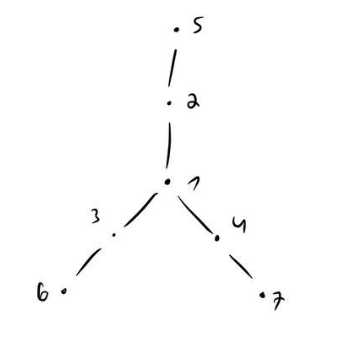
\includegraphics[scale=0.4]{sources/1}
\caption{קומפלקס שלא ניתן לקבל כעצב של קבוצת קטעים במישור.}
\label{figure:1}
\end{figure}

יהי
$\mcal{K} = \set{I_i}{i \in [7]}$
אוסף של שבעה קטעים ב־%
$\mbb{R}$.
במקרה זה,
$I_6$
חותך את
$I_3$
שחותך את
$I_1$,
אבל
$I_1$
לא חותך את
$I_6$
אז נקבל קטעים כמו באיור
\ref{figure:2}.
\begin{figure}
\centering
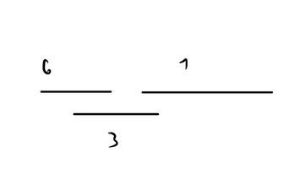
\includegraphics[scale=0.4]{sources/2}
\caption{}
\label{figure:2}
\end{figure}
כעת
$I_2$
חותך את
$I_1$
ואת
$I_5$
שזר ל־%
$I_1$
לכן נקבל קטעים כמו באיור
\ref{figure:3}.
\begin{figure}
\centering
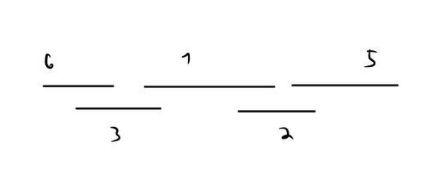
\includegraphics[scale=0.4]{sources/3}
\caption{}
\label{figure:3}
\end{figure}
אז
$I_4$
שחותך את
$I_1$
חייב להיות בין
$I_3, I_2$
אבל אז
$I_4 \subseteq I_!$
ולכן
$I_7$
שחותך את
$I_4$
חותך גם את
$I_1$.
ראו איור
\ref{figure:4}.
\begin{figure}
\centering
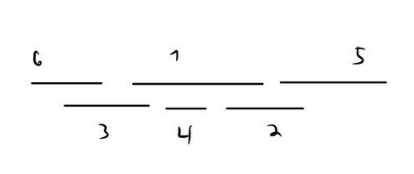
\includegraphics[scale=0.4]{sources/4}
\caption{}
\label{figure:4}
\end{figure}
\end{remark}

\begin{proof}
לכל
$\sigma \in N\prs{\mcal{K}}$
נבחר
$p_\sigma \in \bigcap_{i \in \sigma} K_i$.
נגדיר
\[\text{.} P_i \ceq \conv\set{p_\sigma}{i \in \sigma \in N\prs{\mcal{K}}}\]
נשים לב שאם
$i \in \sigma$
אז
$p_\sigma \in K_i$.
לכן
$P_i \subseteq K_i$.
לכן
$N\prs{\mcal{P}} \subseteq N\prs{\mcal{K}}$.
מאידך, אם
$\sigma \in N\prs{\mcal{K}}$
אז
$p_\sigma \in \bigcap_{i \in \sigma} P_i$
ולכן
$\sigma \in N\prs{\mcal{P}}$.
\end{proof}

\begin{corollary}\label{corollary:disjoint_halfplanes}
תהיינה
$K_1, \ldots, K_m$
קומפקטיות קמורות עבורן
$\bigcap_{i \in [m]} K_i = \ns$.
אזי קיימים חצאי מרחבים
$D_1, \ldots, D_m$
כך שמתקיים
$K_i \subseteq D_i$
לכל
$i \in [m]$,
וגם
$\bigcap_{i \in [m]} D_i = \ns$.
\end{corollary}

\begin{proof}
נוכיח באינדוקציה על
$\ell$
שקיימים
$D_1, \ldots, D_\ell$
עבורם
$K_i \subseteq D_i$
וגם
\[\text{.} D_1 \cap \ldots \cap D_\ell \cap K_{\ell + 1} \cap \ldots \cap K_m = \ns\]
נניח שהוכחנו עבור
$\ell < m$
ונוכיח עבור
$\ell+1$
(זה כולל את מקרה הבסיס).
אז
\begin{align*}
D_1 \cap \ldots \cap D_\ell \cap K_{\ell + 1} \cap \ldots \cap K_m = \ns
\end{align*}
כלומר
\begin{align*}
K_{\ell+1} \cap \prs{D_1 \cap \ldots \cap D_{\ell} \cap K_{\ell + 2} \cap \ldots \cap K_m} = \ns
\end{align*}
ולכן קיים
$H_{u,\alpha}^+$
עבורו
$K_{\ell+1} \subseteq H_{\u,\alpha}^+$
וגם
\[\text{.} D_1 \cap \ldots \cap D_\ell \cap K_{\ell+2} \cap \ldots \cap K_m \subseteq \mrm{int}H_{u,\alpha}^-\]
כלומר,
\[\text{.} D_1 \cap \ldots \cap D_\ell \cap K_{\ell+2} \cap \ldots \cap K_m \cap H_{u,\alpha}^+ = \ns\]
ניקח
$D_{\ell+1} \ceq H_{\u,\alpha}^+$.
\end{proof}

\begin{proof}[\ref{theorem:colourful-helly}]
בלי הגבלת הכלליות, מטענה
\ref{proposition:polytopes-nerve}
אפשר להניח ש־%
$K_{i,j}$
קומפקטיות לכל
$K_{i,j} \in \mcal{K}_i$.

לפי
\ref{corollary:disjoint_halfplanes}
קיימים חצאי מרחבים
$D_{i,j}$
כך ש־%
$K_{i,j} \subseteq D_{i,j}$
לכל
$K_{i,j} \in \mcal{K}_i$
וכך שמתקיים
$\bigcap_{j} D_{i,j} = \ns$.
נציג
\[\text{.} D_{i,j} = H_{u_{i,j}, \alpha_{i,j}}^+ = \set{v \in \mbb{R}^d}{v \cdot u_{i,j} \geq \alpha_{i,j}}\]
יהי
$w_{i,j} = \prs{u_{i,j}, -\alpha_{i,j}} \in \mbb{R}^{d+1}$.

נשים לב שמתקיים
\[\bigcap_j H_{w_{i,j}, 0}^+ \cap \prs{\mbb{R}^d \times \set{1}} = \ns\]
אם
$v = \prs{v', v_{d+1}}$
בחיתוך הנ"ל אז
$w_{i,j} \cdot \prs{v', v_{d+1}} \geq 0$
ומצד שני
$v_{d+1} = 1$.
אז
\begin{align*}
v' \cdot u_{i,j} + \prs{-\alpha_{i,j}} \cdot 1 \geq 0
\end{align*}
ולכן
$v' \cdot u_{i,j} \geq \alpha_{i,j}$
לכל
$j$.
אז
$v' \in D_{i,j}$
לכל
$j$,
בסתירה לכך שמתקיים
\[\text{.} \bigcap_j D_{i,j} = \ns\]
לכן, לפי
\ref{lemma:pos-conditions}
מתקיים
\[\prs{\vec{0}, -1} \in \mrm{pos}\set{w_{i,j}}_j\]
לכל
$i \in [d+1]$.
לפי קרתיאודורי הצבעוני עבור
\textenglish{pos}
קיימת בחירה
$w_{1, j_1}, w_{2,j_2}, \ldots, w_{d+1, j_{d+1}}$
כך שמתקיים
\[\text{.} \prs{\vec{0},-1} \in \mrm{pos}\set{w_{i,j_i}}_{i \in [d+1]}\]

לפי
\ref{lemma:pos-conditions}
נקבל כי
\[\text{.} \bigcap_{i \in \brs{d+1}} H_{w_{i,j_i},0}^+ \cap \prs{\mbb{R}^d \times \set{1}} = \ns\]
אז
\[\bigcap_{i \in [d+1]} K_{i, j_i} \subseteq \bigcap_{i \in [d+1]} D_{i, j_i} = f\bigcap_{i \in \brs{d+1}} H_{u_{i,j_i, \alpha_{i, j_i}}}^+ = \ns\]
כיוון שאם
$z \in \bigcap_{i \in [d]} H_{u_{i,j_i}, \alpha_{i,j_i}}^+$
אז
$z \cdot u_{i,j_i} \geq \alpha_{i,j_i}$
לכל
$i$
ואז
\begin{align*}
\prs{z,1} \cdot w_{i,j_i} &= \prs{z,1} \cdot \prs{u_{i,j_i}, -\alpha_{i,j_i}}
\\&= z \cdot u_{i, j_i} - \alpha_{i,j_i} > 0
\end{align*}
ונקבל כי
\[\prs{z,1} \in \bigcap_{i \in [d+1]} H_{w_{i,j_i}}^+ \cap \prs{\mbb{R}^d \times \set{1}}\]
בסתירה לביטוי קודם.
קיבלנו
\[\bigcap_{i \in [d+1]} K_{i, j_i} = \ns\]
בסתירה להנחה.
\end{proof}

\begin{theorem}[רדון]
תהיינה
$u_1, \ldots, u_{d+2} \in \mbb{R}^d$.
קיימת חלוקה
$\brs{d+2} = I_1 \sqcup I_2$
עבורה
\begin{align*}
\text{.} \conv\set{u_i}_{i \in I_1} \cap \conv\set{u_i}_{i \in I_2} = \ns
\end{align*}
\end{theorem}

נשאל מה מספר הנקודות המינימלי
$m$
כך שלכל
$u_1, \ldots, u_m \in \mbb{R}^2$
תהיה חלוקה
$\brs{m} = I_1 \sqcup I_2 \sqcup I_3$
עבורה
\[\text{.} \bigcap_{j \in [3]} \conv\set{u_i}_{i \in I_j} \neq \ns\]

\begin{theorem}[טברברג] \label{theorem:tverberg}
אם
$u_1, \ldots, u_m \in \mbb{R}^d$
וגם
$m \geq \prs{d+1}\prs{k-1} + 1$
אז יש חלוקה
$\brs{m} = \bigsqcup_{j \in [k]} I_j$
וגם
\[\text{.} \bigcap_{j \in [k]} \conv\set{u_i}_{i \in I_j} \neq \ns\]
\end{theorem}

\begin{remark}
על ידי הסתכלות על
$d+1$
קבוצות בגודל
$k-1$
 של נקודות קרובות (או שוות זאת לזאת, לא הנחנו שה־%
$u_i$
שונות)
  ב־%
$\mbb{R}^d$
אפשר לראות שהחסם התחתון במשפט טברברג אופטימלי, כיוון שבמקרה זה אין חלוקת
$k$%
־טברברג.
\end{remark}

%lecture 27.4.2021

בהוכחת משפט טברברג נרצה לעבוד במרחב
$\prs{k-1}\prs{d+1}$%
־מימדי.
נזכיר כי
$M_{k \times \ell}\prs{\mbb{R}} \cong \mbb{R}^k \tensor \mbb{R}^\ell$
מרחב ממימד
$k\ell$.
בהינתן
$u \in \mbb{R}^k, v \in \mbb{R}^\ell$
נגדיר
\[\text{.} u \tensor v \ceq u v^T = \pmat{u_1 v_1 & & \cdots & & u_\ell v_\ell \\ & & & & \\ \vdots & & & & \vdots \\ & & & & \\ u_k v_1 & & \cdots & & u_k v_\ell}\]

\begin{proposition}
נניח כי
$v_1, \ldots, v_k \in \mbb{R}^{k-1}$
מקיימים
\[\sum_{i \in [k]} v_i = 0\]
ושזאת התלות היחידה ביניהם.
למשל אפשר לקחת
$v_1, \ldots, v_{k-1}$
בסיס ל־%
$\mbb{R}^{k-1}$
ו־%
$v_k = -\prs{v_1 + \ldots + v_{k-1}}$
(זה בעצם המקרה הכללי).
נניח גם כי
$u_1, \ldots, u_k \in \mbb{R}^{N}$
מקיימים
\[\text{.} \sum_{i \in [k]} u_i \tensor v_i = 0 \in \mbb{R}^N \tensor \mbb{R}^{\prs{k-1}} \cong M_{N \times \prs{k-1}}\]
אז
$u_i = u_j$
לכל
$i,j \in [k]$.
\end{proposition}

\begin{remark}
ברור שאם
$u_i = u_j$
לכל
$i,j \in [k]$
אז
\[\text{.} \sum_{i \in \brs{k}} u_i \tensor v_i = u \tensor \sum_{i \in \brs{k}} v_i = u \tensor 0 = 0\]
\end{remark}

\begin{proof}
יהי
$z \in \mbb{R}^N$.
מתקיים
\begin{align*}
0 &= z^T \cdot \prs{\sum_{i \in [k]} u_i v_i^T} = \sum_{i \in [k]} \prs{z^T \cdot u_i} \cdot v_i^T
\end{align*}
לכן
$z^T \cdot u_i = z^T \cdot u_j$
לכל
$i,j \in [k]$.
זה נכון לכל
$z \in \mbb{R}^N$
לכן
$z^T \prs{u_i - u_j} = 0$
לכל
$z \in \mbb{R}^n$
ולכן
$u_i = u_j$.
\end{proof}

\begin{proof}[\ref{theorem:tverberg}]
על ידי הוספת רכיב לכל
$u_i$
אפשר להניח כי
$u_1, \ldots, u_m \in \mbb{R}^{d+1}$
וגם ש־%
$u_i \cdot \1 = 1$
כאשר
$\1 = \pmat{1 \\ 1 \\ \vdots \\ 1 \\ 1} \in \mbb{R}^{d+1}$.
יהיו
$v_1, \ldots, v_k \in \mbb{R}^{k-1}$
עבורם
$\sum_{i \in [k]} v_i = 0$
וזאת התלות היחידה ביניהם.
נשתמש בקרתיאודורי הצבעוני עבור
$\mbb{R}^{\prs{d+1}\prs{k-1}} \cong M_{\prs{d+1} \times \prs{k-1}}\prs{\mbb{R}}$.
לכל
$i \in [m]$
תהי
\[\text{.} A_i = \set{u_i \tensor v_j}{j \in [k]} \subseteq \mbb{R}^{\prs{d+1}\prs{k-1}}\]

מתקיים
$0 \in \bigcap_{i \in [m]} \conv\prs{A_i}$
כי
\[\text{.} 0 = u_i \tensor 0 = u_i \tensor \prs{\frac{1}{k} \sum_{j \in [k]} v_j} = \frac{1}{k} \sum_{j \in [k]} u_i \tensor v_j\]
לפי קרתיאודורי הצבעוני, לכל
$i \in \brs{m}$
קיים
$j_i \in [k]$
כך שמתקיים
\[\text{.} 0 \in \conv\set{u_i \tensor v_{j_i}}{i \in [m]}\]
אז יש
$\lambda_i \geq 0$
המקיימות
\begin{align*}
\sum_{i \in [m]} \lambda_i &= 1 \\
\text{.} \sum_{i \in [m]} \lambda_i \prs{u_i \tensor v_{j_i}} &= 0
\end{align*}
אבל אם נסמן
\[I_j \ceq \set{i \in [m]}{j_i = j}\]
נקבל
\begin{align*}
\text{.}  \sum_{j \in [k]} \prs{\sum_{i \in I_j} \lambda_i u_i} \tensor v_j &= \sum_{i \in [m]} \lambda_i \prs{u_i \tensor v_{j_i}} = 0
\end{align*}
לפי הטענה, קיים
$w \in \mbb{R}^d$
כך שלכל
$j \in [k]$
מתקיים
\[\text{.} w = \sum_{i \in I_j} \lambda_i u_i\]
אז
\[w \cdot \1 = \sum_{i \in I_j} \lambda_i \cdot \prs{u_i \cdot \1} = \sum_{i \in I_j} \lambda_i\]
ולכן
\begin{align*}
\frac{w}{w \cdot \1} &= \sum_{i \in I_j} \frac{\lambda_i}{w \cdot \1} \cdot u_i
\\&= \sum_{i \in I_j} \frac{\lambda_i}{\sum_{t \in I_j} \lambda_t} u_i
\\&\in \conv\set{u_i}_{i \in I_j}
\end{align*}
כנדרש.
\end{proof}

\subsection{משפט הנקודה הכבדה של
\textenglish{Barany}}

\begin{theorem}[\text{Barany}]
לכל
$d \geq 1$
יש קבוע
$C_d > 0$
כך שלכל
$u_1, \ldots, u_n \in \mbb{R}^d$
יש
$\mcal{F} \subseteq \binom{\brs{n}}{d+1}$
עבורה
$\abs{\mcal{F}} > C_d \binom{n}{d+1}$
וכך שקיימת
\[\text{.} p \in \bigcap_{F \in \mcal{F}} \conv\set{u_i}{i \in F}\]
\end{theorem}

\begin{proof}
נגדיר את
$k$
להיות השלם המקסימלי עבורו
$\prs{k-1}\prs{d+1} + 1 \leq n$.
כלומר,
$k = \floor{\frac{n-1}{d+1}} + 1$.

נניח כי
$k \geq d+1$.
לפי משפט
\ref{theorem:tverberg}
נחלק את
$\brs{n}$
לקבוצות זרות
$I_1, \ldots, I_k$
כך שיש
\[\text{.} p \in \bigcap_{j \in [k]} \conv\set{u_i}_{i \in I_j}\]
לכל בחירה
$\alpha_1 < \ldots < \alpha_{d+1}$
של איברים ב־%
$\brs{k}$
מתקיים
\[\text{.} p \in \bigcap_{t \in \brs{d+1}} \conv\set{u_i}{i \in I_{\alpha_t}}\]
לפי קרתיאודורי הצבעוני יש
$d+1$
נקודות, אחת מכל
$\set{u_i}_{i \in I_{\alpha_t}}$
כך ש־%
$p$
בקמור שלהן.
נסמן את קבוצת האינדקסים של נקודות אלו ב־%
$F_{\alpha}$
כאשר
$\alpha = \prs{\alpha_1, \ldots, \alpha_{d+1}}$.
אם
$\alpha \neq \beta$
נקבל
$F_\alpha \neq F_\beta$
ולכן
\[\mcal{F} \ceq \set{F_{\alpha}}{1 \leq \alpha_1 < \ldots < \alpha_{d+1} \leq k}\]
קבוצה מגודל
$\binom{k}{d+1}$.
אז
\begin{align*}
\abs{\mcal{F}}
&=
\binom{k}{d+1}
\\&=
\binom{\floor{\frac{n-1}{d+1}} + 1}{d+1}
\\&\geq
\binom{\floor{\frac{n-1}{d+1}}}{d+1}
\\&\geq
\frac{\prs{\floor{\frac{n-1}{d+1}} - d + 1}^{d+1}}{\prs{d+1}!}
\\&\geq \frac{\prs{\frac{n-1}{d+1} - d}^{d+1}}{\prs{d+1}!}
\\&= \frac{\prs{n-d^2 - d - 1}^{d+1}}{\prs{d+1}^{d+1} \prs{d+1}!}
\\&\geq \frac{n^{d+1} - \prs{d+1}\prs{d^2 + d + 1} n^d}{\prs{d+1}^{d+1} \prs{d+1}1}
\\&= \frac{1}{\prs{d+1}^{d+1}} \brs{\frac{n^{d+1}}{\prs{d+1}!} - \frac{\prs{d+1}\prs{d^2 + d + 1}}{\prs{d+1}!} n^d}
\\&\geq \frac{1}{\prs{d+1}^{d+1}} \prs{\binom{n}{d+1} - \lambda_d n^d}
\\&\geq \frac{1}{2 \prs{d+1}^{d+1}} \binom{n}{d+1}
\end{align*}
עבור קבוע
$\lambda_d$
וכאשר האי־שוויון האחרון נכון עבור
$n$
גדול מספיק.
נבחר
$C_d = \frac{1}{2 \prs{d+1}^{d+1}}$.
\end{proof}

\begin{remark}
בהינתן
$d$
אפשר לשאול מה הסופרמום
$\theta_d$
של ערכים
$\theta$
עבורם לכל
$n$
נקודות ב־%
$\mbb{R}^d$
יש
$p$
נקודות בלפחות
$\theta \cdot \binom{n}{d+1}$
מהסימפלקסים על ידי הנקודות.

עבור
$d \in \set{1,2}$
ידועים הערכים של
$\theta_d$.
עבור
$d > 2$
זאת בעיה פתוחה.
\end{remark}

%date 28.4

\subsection{רשתות
$\eps$
חלשות}

תהי
$\mcal{K}$
משפחה של קבוצות מדידות במרחב הסתברות
$\prs{\Omega, B, \mu}$.
נעיין בקבוצה
\[\text{.} A_{\eps} \ceq \set{K \in \mcal{K}}{\mu\prs{K} \geq \eps}\]
נרצה למצוא
$S \subseteq \Omega$
מגודל מינימלי כך ש־%
$S \cap K \neq \ns$
לכל
$K \in A_\eps$.

\begin{example}
יהי
$\Omega = \mbb{R}$
עם מידת הסתברות
$\mu$
המתוארת באופן הבא.
יהיו
$u_1 \leq \ldots \leq u_n$
נקודות ב־%
$\mbb{R}$.
נגדיר
\begin{align*}
\mu \ceq \frac{1}{n} \sum_{i \in [n]} \delta_{u_i}
\end{align*}
כאשר
$\delta_{u_i}$
מידת דיראק של
$u_i$.
נשאל האם יש
$S \subseteq \Omega$
סופית מגודל קטן מ־%
$f\prs{\eps}$
עבור
$f\prs{\eps}$
קבוע כלשהו התלוי באפסילון וכך שכל
$K \in A_\eps$
חותכת את
$S$.

תהי
\[\text{.} S = \set{u_{i \floor{\eps n}}}{i \in \floor{\frac{1}{\eps}}}\]
אז לכל קטע
$K$
עם
$\mu\prs{K} \geq \eps$
מתקיים
$K \cap S \neq \ns$.
אבל גם
$\abs{S} \leq \floor{\frac{1}{\eps}}$.
\end{example}

\begin{theorem}
תהא
$\mu$
מידת הסתברות דיסקרטית על
$\mbb{R}^d$
הנקבעת על ידי
$\set{u_i}_{i \in [n]} \subseteq \mbb{R}^d$
ו־%
\[\text{.} \mu\prs{A} = \frac{1}{n} \abs{\set{i}{u_i \in A}}\]
תהא
$\mcal{K}$
משפחת הקבוצות הקמורות ב־%
$\mbb{R}^d$.
אז יש
$S \subseteq \mbb{R}^d$
עם
$\abs{S} \leq \lambda_d \cdot \prs{\frac{1}{\eps}}^{d+1}$
עבורה
$S \cap K \neq \ns$
לכל
$K$
המקיימת
$\mu\prs{K} \geq \eps$.
\end{theorem}

\begin{proof}
לכל
$K \in \mcal{K}$
עבורה
$\mu\prs{K} \geq \eps$
תהא
$I_K \ceq \set{i}{u_i \in K}$.
אז
$\abs{I_k} \geq \eps n$.
לפי משפט הנקודה הכבדה, יש
$\mcal{F}_K \subseteq \binom{I_k}{d+1}$
עם
\[\abs{\mcal{F}_K} \geq c_d \cdot \binom{\abs{I_k}}{d+1} \geq c_d \binom{\eps n}{d+1}\]
וכך שקיימת
\[\text{.} p_K \in \bigcap_{F \in \mcal{F}_K} \conv\set{u_i}_{i \in F}\]
נבחר משפחה מקסימלית
$K_1, \ldots, K_r$
מתוך ה־%
$K \in \mcal{K}$
המקיימות
$\mu\prs{K} \geq \eps$
כך ש־%
$\mcal{F}_{K_1}, \ldots, \mcal{F}_{K_r}$
זרות בזוגות.

אז
\begin{enumerate}
\item $S = \ceq \set{p_{K_1}, \ldots, p_{K_r}}$
מקיימת
$S \cap K \neq \ns$
לכל
$K \in \mcal{K}$
עבורה
$\mu\prs{K} \geq \eps$:

תהא
$K$
כזאת. אז ממקסימליות
$K_1, \ldots, K_r$
נובע שקיים
$i \in \brs{r}$
עבורו
$\mcal{F}_K \cap \mcal{F}_{K_i} \neq \ns$.
אז קיימת
$F \in \mcal{F}_K \cap \mcal{F}_{K_i}$.
כעת,
$\set{u_j}{j \in F} \subseteq K \cap K_i$.
לכן
\[\text{.} p_{K_i} \in \conv\set{u_j}{j \in F} \subseteq K\]

\item נותר להראות ש־%
$r$
תלוי ב־%
$\eps$
בלבד.
מתקיים
\begin{align*}
\bigsqcup_{i \in [r]} \mcal{F}_{K_i} \subseteq \binom{\brs{n}}{d+1}
\end{align*}
לכן
\[\text{.} \sum_{i \in [r]} \abs{\mcal{F}_{K_i}} \\leq \binom{n}{d+1}\]
אבל
\[r \cdot c_d \binom{\floor{\eps} n}{d+1} \leq \sum_{i \in [r]} \abs{\mcal{F}_{K_i}} \leq \binom{n}{d+1}\]
ולכן
\begin{align*}
r &\leq \frac{\binom{n}{d+1}}{c_d \binom{\floor{\eps}n}{d+1}}
\\&\leq \frac{\frac{n^{d+1}}{\prs{d+1}!}}c_d \frac{\prs{\prs{\eps n  - d}^{d+1}}}{\prs{d+1}!}
\\&= \frac{1}{c_d} \prs{\frac{n}{\eps n - d}}^{d+1}
\\ \text{.} \hphantom{r} &\xrightarrow{n\to\infty} \frac{1}{c_d} \prs{\frac{1}{\eps}}^{d+1}
\end{align*}
\end{enumerate}
\end{proof}

\chapter{פיאונים}

\section{(קו)הומולוגיה}

\subsection{קוהומולוגיה}

לפעמים נרצה לפתור מערכת משוואות כאשר מימד מרחב הפתרונות אינסופי. נרצה הרבה פעמים לסנן את הפתרונות הטריוויאליים ולהישאר עם פתרונות אמיתיים.

\begin{example}
יהי
$\Omega \subseteq \mbb{R}^2$
תחום פתוח.
נחפש את אוסף השדות הוקטוריים
\[F\prs{x,y} = \prs{P\prs{x,y}, Q\prs{x,y}}\]
על
$\Omega$:
\[\text{.} W \ceq \set{\prs{P,Q}}{\frac{\del Q}{\del x} = \frac{\del P}{\del y}}\]
זה מרחב וקטורי מעל
$\mbb{R}$.

בעצם, יש כאן הרבה פתרונות טריוויאליים. מתקיים
\[\text{.} W \ceq \set{\prs{P,Q}}{\nabla \times \prs{P,Q} = 0}\]
אז
$W$
מכיל את כל השדות המשמרים,
$\prs{P,Q} = \nabla g$.
כלומר, אם
$P = \frac{\del g}{\del x}$
וגם
$Q = \frac{\del g}{\del y}$
אז
\[\text{.} \frac{\del Q}{\del x} - \frac{\del P}{\del y} = \frac{\del^2 g}{\del x \del y} - \frac{\del^2 g}{\del y \del x} = 0\]

נגדיר
\[W_0 \ceq \set{\nabla g}{\text{$g\prs{x,y}$ is smooth on $\omega$}}\]
ונקרא לאלו הפתרונות הטריוויאליים. נרצה לשאול האם יש פתרונות שאינם טריוויאליים.
לכל
$\Omega$
כזה מתקיים
$W_{0,\Omega} \subseteq W_\Omega$.

\begin{itemize}
\item אם
$\Omega = \mbb{R}^2$
אין פתרונות נוספים.

\item אם
$\Omega = \mbb{R}^2 \setminus \set{0,0}$
אז
$W_{0,\Omega} \neq W_{\Omega}$.
אכן,
\[\prs{P,Q} = \frac{\prs{-y,x}}{x^2 + y^2}\]
אינו מהצורה
$\nabla g$.
אם הוא היה, עבור
$\gamma\prs{t} = \prs{\cos t, \sin t}$
היינו מקבלים
\begin{align*}
0 &= g\prs{\gamma\prs{2 \pi}} - g\prs{\gamma\prs{0}}
\\&=
\int_\gamma \nabla g
\\&=
\int_\gamma P \diff x + Q \diff y
\\&=
\int_\gamma \frac{-y \diff x + x \diff y}{x^2 + y^2}
\\&= 2 \pi
\end{align*}
בסתירה.
\end{itemize}
\end{example}

\begin{definition}[קוהומולוגיה ראשונה]
מרחב הפתרונות "שאינם טריוויאליים" הוא
$H^1\prs{\Omega, \mbb{R}} \ceq W_\Omega/W_{0,\Omega}$.
נקרא למרחב זה
\emph{הקוהומולוגיה הראשונה של
$\Omega$}
עם מקדמים ב־%
$\mbb{R}$.
כאן
$\dim H^1\prs{\Omega, \mbb{R}}$
יהיה מספר ה"חורים" ב־%
$\Omega$.
\end{definition}

\begin{example}
במקרה ש־%
$\Omega$
קבוצה דיסקרטית מגודל
$3$
נקבל
$\dim H^1\prs{\Omega, \mbb{R}}$.
\end{example}

\subsection{הומולוגיה}

עבור מרחב טופולוגי
$X$
ושדה
$\mbb{F}$
נרצה להגדיר חבורות הומולוגיה
$H_k\prs{X;\mbb{F}}$
שמתאר את החורים ה־%
$k$%
־מימדיים ב־%
$X$.

\begin{definition}[קומפלקס סימפליציאלי מופשט]
\emph{קומפלקס סימפליציאלי מופשט}
הוא קבוצת קודקודים
$V$
וקבוצה
$X \subseteq \mcal{P}\prs{V}$
עבורה אם
$\sigma \in X$
וגם
$\tau \subseteq \sigma$
אז
$\tau \in X$.
נגדיר את המימד של
$X$
להיות
\[\dim X \ceq \max\set{\dim \sigma}{\sigma \in X}\]
כאשר
$\dim \sigma \ceq \abs{\sigma} - 1$.
\end{definition}

\begin{definition}[סימפלקס גיאומטרי]
\emph{סימפלקס גיאומטרי}
ממימד
$k$
הוא קבוצה מהצורה
$\conv\set{u_0, \ldots, u_k}$
כאשר
$u_0, \ldots, u_k$
בלתי־תלויים אפינית.
\end{definition}

\begin{definition}[קומפלקס סימפליציאלי גיאומטרי]
\emph{קומפלקס סימפליציאלי גיאומטרי}
הוא אוסף
$Y$
של סימפלקסים גיאומטריים ב־%
$\mbb{R}^N$
כך שמתקיימות התכונות הבאות.
\begin{enumerate}
\item אם
$\sigma \in Y$
ו־%
$\tau \leq \sigma$
פאה של
$\sigma$
אז
$\tau \in Y$.
\item אם
$\sigma_1, \sigma_2 \in Y$
אז
$\sigma_1 \cap \sigma_2$
פיאה (אולי ריקה) של
$\sigma_1, \sigma_2$.
\end{enumerate}
\end{definition}

\begin{definition}[מימוש של קומפלקס סימפליציאלי מופשט]
קומפלקס סימפליציאלי גיאומטרי
$Y$
עם קבוצת קודקודים
$u_1, \ldots, u_m$
הוא
\emph{מימוש גיאומטרי של קומפלקס סימפליציאלי מופשט
$X$
עם קבוצת קודקודים
$v_1, \ldots, v_m$}
אם קיימת העתקה
\begin{align*}
\phi \colon \set{u_i}{i \in [m]} \to \set{x_i}{i \in [m]} \\
v_i &\mapsto u_i
\end{align*}
עבורה
$\set{u_{i_0}, \ldots, u_{i_k}} \in X$
אם ורק אם
$\conv\prs{u_{i_0}, \ldots, u_{i_k}} \in Y$.
\end{definition}

\begin{example}
\begin{enumerate}
\item לגרף
$K_4$
יש מימוש ב־%
$\mbb{R}^2$.
המרחב באיור
%TODO add fig 1.1
אינו מימוש כיוון שחיתוך שני האלכסונים אינו סימפלקס.
המרחב באיור
%TODO add fig 1.2
לעומת זאת הוא אכן שיכון גיאומטרי.

\begin{figure}
\centering
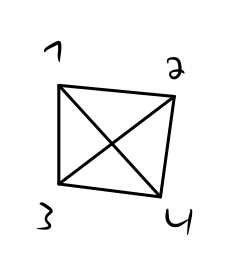
\includegraphics[scale=0.4]{sources/1.1}
\caption{קומפלקס שלא ניתן לקבל כעצב של קבוצת קטעים במישור.}
\label{figure:1.1}
\end{figure}

\begin{figure}
\centering
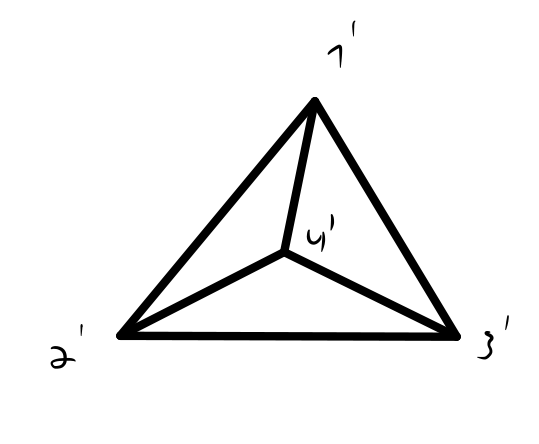
\includegraphics[scale=0.4]{sources/1.2}
\caption{קומפלקס שלא ניתן לקבל כעצב של קבוצת קטעים במישור.}
\label{figure:1.2}
\end{figure}

\item לגרף
$K_5$
אין מימוש ב־%
$\mbb{R}^2$,
אבל יש מימוש ב־%
$\mbb{R}^3$.
למעשה, כל גרף אפשר לממש ב־%
$\mbb{R}^3$.
\end{enumerate}
\end{example}

\begin{proposition}
יהי
$X$
קומפלקס סימפליציאלי אבסטרקטי על קבוצת קודקודים
$\brs{n}$
ונניח כי
$\dim X = d$.
אזי, יש ל־%
$X$
מימוש גיאומטרי ב־%
$\mbb{R}^{2d + 1}$.
\end{proposition}

\begin{proof}
נבחר
$u_1, \ldots, u_m \in \mbb{R}^{2d+1}$
שהן במצב כללי אפיני, כלומר כל
$2d + 2$
מהן בלתי־תלויות אפינית. למשל, אם
$d=1$,
כל
$4$
קודקודים יוצרים טטרהדר לא־מנוון.

באופן כללי, ב־%
$\mbb{R}^N$
יש סדרה (אינסופית) של נקודות
$u_1, u_2, \ldots$
שכל
$N+1$
מהן בלתי־תלויות אפינית. (למשל
$u_j = \prs{j, j^2, \ldots, j^N}$
סדרה כזאת)
נניח שמצאנו את
$u_1, \ldots, u_n$
שהן במצב כללי אפיני.
יש
$\binom{n}{N}$
מרחבים אפיניים שנפרשים אפינית על ידי
$N$
מתוך ה־%
$\prs{u_i}_{i \in [n]}$,
ולכן אפשר לבחור
$u_{m+1}$
שאינה באף אחד מהם.

\emph{המימוש הגיאומטרי של
$X$}
הוא הקומפלקס הגיאומטרי
$Y$
שסימפלקסיו הם
$\conv\set{u_{i_0}, \ldots, u_{i_p}}$
לכל
$\prs{i_0, \ldots, i_p} \in X$.

ניתן אז להראות כי
$Y$
מקיים את הדרישות.
\end{proof}

\begin{definition}[מימוש גיאומטרי של קומפלקס גיאומטרי]
עבור קומפלקס גיאומטרי
$Y$
נגדיר את
\emph{המימוש הגיאומטרי שלו}
על ידי
\[\text{.} \abs{Y} = \bigcup_{\sigma \in Y} \sigma\]
\end{definition}

\begin{proposition}
יהי
$X$
קומפלקס סימפליציאלי אבסטרקטי עם
$Y_1, Y_2$
מימושים גיאומטריים של
$X$.
אז
$\abs{Y_1} \cong \abs{Y_2}$.
\end{proposition}

\begin{proof}
תהי
$X \subseteq \mcal{P}\prs{\brs{n}}$
ויהיו
$Y_1, Y_2$
מימושים על קודקודים
$u_1, \ldots, u_n \in \mbb{R}^{N_1}$
ו־%
$v_1, \ldots, v_n \in \mbb{R}^{N_2}$.
נגדיר
$\phi \colon Y_1 \to Y_2$
על ידי
$\phi\prs{u_i} = v_i$
ואם
$y \in \abs{Y_1}$
נכתוב
\begin{align*}
\sum_{j = 0}^p \lambda_j u_{i_j} = y \in \conv\set{u_{i_0}, \ldots, u_{i_p}}
\end{align*}
עבור
$\lambda_j \geq 0$
המקיימות
$\sum_{j=0}^p \lambda_j = 1$
ונגדיר
\[\text{.} \phi\prs{y} = \sum_{j=0}^p \lambda_j v_{i_j}\]
למשל, במקרה
$X = \set{\set{1}, \set{2}, \set{3}, \set{1,2}, \set{1,3}}$
ההעתקה
$\phi \colon Y_1 \to Y_2$
ממשיכה לינארית מהקטע בין
$u_1, u_2$
לקטע בין
$v_1, v_2$.

אז
$\phi$
הומיאומורפיזם
$Y_1 \cong Y_2$.
\end{proof}

\begin{corollary}
אפשר לזהות קומפלקס סימפליציאלי אפיני עם מימוש כלשהו שלו ב־%
$\mbb{R}^N$
עד כדי הומיאומורפיזם.
\end{corollary}

מרחבים קומפקטיים
\textit{סבירים}
ניתן לשלש במובן שהם הומיאומורפיים לקומפלקסים סימפליציאליים סופיים.

\begin{notation}
נסמן
$\Delta_{n-1} = 2^{\brs{n}}$
כסימפלקס על
$\brs{n}$.
\end{notation}

\begin{notation}[השלד ה־%
$k$%
־מימדי]
\emph{השלד ה־%
$k$%
־מימדי של
$\Delta_{n-1}$}
הוא
\[\text{.} \Delta_{n-1}^{\prs{k}} \ceq \set{\sigma \in \Delta_{n-1}}{\dim \sigma \leq k}\]
\end{notation}

\begin{example}
הספירה
$S^n$
ניתנת לשילוש.
לכל
$n \in \mbb{N}_+$
מתקיים
\[\text{.} S^{n-2} \cong \Delta_{n-1}^{\prs{n-2}}\]
\end{example}

\begin{example}
אפשר לשלש גם את הטורוס
$S^1 \times S^1$.
נסתכל על הטורוס כהדבקה של ריבוע על הצלעות. ניתן לחלק אותו באופן
%TODO add fig 1.3
\end{example}

\subsubsection{הגדרת הומולוגיה סימפליציאלית}

יהי
$X$
קומפלקס סימפליציאלי (אבסטרקטי) על קודקודים
$V$
ונניח כי
$V$
קבוצה סדורה לינארית.
יהי
$X\prs{k}$
אוסף הפיאות ה־%
$k$%
־מימדיות של
$X$.
יהי
$X^{\prs{k}} \ceq \set{\sigma \in X}{\dim \sigma \leq k}$
\emph{השלד ה־%
$k$%
־מימדי של
$X$}.
נייצג פיאה
$k$%
־מימדית
$\set{v_0, \ldots, v_k}$
על ידי קבוצה סדורה
$\brs{v_0, \ldots, v_k}$
כאשר
$v_0 < \ldots < v_k$.

\begin{definition}
יהי
$\mbb{F}$
שדה. נגדיר את
$C_n\prs{X,\mbb{F}}$
להיות המרחב הוקטורי מעל
$\mbb{F}$
הנפרש על ידי הסימלפקסים
$\brs{v_0, \ldots, v_k} \in X\prs{k}$.
\end{definition}

\begin{example}
יהי
$X$
כבאיור
%TODO add fig 1.4

אז למשל
\[17 \brs{1} + 5 \brs{3} - 2 \brs{4} \in C_0\prs{X,\mbb{F}}\]
והמרחב
$C_k\prs{X}$
ממימד
$\abs{X\prs{k}}$.
למשל גם
$1 \cdot \brs{3,4} + \prs{-1}\brs{2,3}$.
\end{example}

\begin{remark}
כרגע, נסתכל רק על סימפלקסים
$\brs{v_0, \ldots, v_k}$
כאשר
$v_0 < v_1 < \ldots < v_k$.
בהמשך נתייחס גם לשינוי סדר של זה.
\end{remark}

\begin{definition}
נסמן
$\brs{\ns} = *$
ונגדיר
\[\text{.} C_{-1} \prs{X} = \mbb{F} \cdot * \cong \mbb{F}\]
\end{definition}

\begin{definition}[העתקת שפה]
עבור
$k \geq 1$
נגדיר את
\emph{העתקת ה־%
$k$%
־שפה}
\[\del_k \colon C_k\prs{X} \to C_{k-1} \prs{X}\]
על איברי הבסיס על ידי
\[\delta_k \prs{\brs{v_0, \ldots, v_k}} = \sum_{j=0}^k \prs{-1}^j \brs{v_0, \ldots, \hat{v}_j, \ldots, v_k}\]
כאשר
$\hat{v}_j$
סימון לכך שזה איבר שמושמט מהביטוי.
\end{definition}

\begin{example}
נסתכל על הסימלפקס
$\brs{v_0, v_1}$.
אז
\[\text{.} \del_1\prs{\brs{v_0, v_1}} = \sum_{j=0}^1 \prs{-1}^j \brs{v_0, \ldots, \hat{v}_j, v_1} = \brs{v_1} - \brs{v_0}\]
\end{example}

\begin{example}
נסתכל על
$\brs{v_0, v_1, v_2}$.
אז
\begin{align*}
\text{.} \del_2 \prs{\brs{v_0, v_1, v_2}} = \brs{v_1, v_2} - \brs{v_0, v_2} + \brs{v_0, v_1}
\end{align*}
ניתן לחשוב על כך כבאיור
%TODO 1.5
\end{example}

\begin{definition}[$k$%
־מחזורים]
נסמן
\[\text{.} Z_k\prs{X} \ceq \set{c \in C_k\prs{X}}{\del_k c = 0}\]
\end{definition}

\begin{example}
נסתכל על איור
%TODO 1.6
מתקיים
\begin{align*}
\del_2\prs{\brs{1,2,3}}
&=
\del_1\prs{\brs{1,2} + \brs{2,3} - \brs{1,3}}
\\&= \del_1\brs{1,2} + \del_1 \brs{2,3} - \del_1\brs{1,3}
\\&= \prs{\brs{2} - \brs{1}} + \prs{\brs{3} - \brs{2}} - \prs{\brs{3} - \brs{1}}
\\ \text{.} \hphantom{\del_!\prs{\brs{1,2} + \brs{2,3} - \brs{1,3}}} &= 0
\end{align*}
וניתן לראות כי
$Z_1\prs{X}$
הוא מעגלים מכוונים בקומפלקס.
\end{example}

\begin{example}
נסתכל על
$X$
שילוש של
$\mbb{T} = S^1 \times S^1$.
אז
\[\del_2 \prs{\sum_{\sigma \in X\prs{2}} \sigma} = 0\]
כיוון שכל צלע תופיע פעמיים בסימנים הפוכים, וכאשר הסימפלקסים באוריינטציה תואמת.
%TODO add 1.7

ניתן בדוגמא זאת לראות גם שמתקיים
$\del_l \circ \del_{k+1} = 0$.
זה בעצם מתקיים באופן כללי יותר.
\end{example}

\begin{proposition}
$\del_k \circ \del_{k+1} = 0$
לכל
$k \in \mbb{N}$.
\end{proposition}

\begin{proof}
מתקיים
\begin{align*}
\del_k \del_{k+1} \brs{v_0, \ldots, v_{k+1}}
&=
\del_k \sum_{i = 0}^{k+1} \prs{-1}^i \brs{v_0, \ldots, \hat{v}_i, \ldots, v_{k+1}}
\\&=
\sum_{i=0}^{k+1} \prs{-1}^i \del_k \brs{v_0, \ldots, \hat{v}_i, \ldots, v_{k+1}}
\\&=
\sum_{i = 0}^{k+1} \prs{-1}^i \prs{\sum_{j = 0}^{i-1} \prs{-1}^j \brs{v_0, \ldots, \hat{v}_j, \ldots, \hat{v}_i, \ldots, v_{k+1}}
+
\sum_{j = i+1}^{k+1} \prs{-1}^{j-1} \brs{v_0, \ldots, \hat{v}_i, \ldots, \hat{v}_j, \ldots, v_{k+1}}}
\\&=
\sum_{\substack{\prs{i,j} \in [k+1]^2 \\ j < i}} \prs{-1}^{i+j} \brs{v_0, \ldots, \hat{v}_j, \ldots, \hat{v}_i, \ldots, V_{k+1}}
+
\sum_{\substack{\prs{i,j} \in [k+1]^2 \\ j > i}} \prs{-1}^{i+j-1} \brs{v_0, \ldots, \hat{v}_i, \ldots, \hat{v}_j, \ldots, V_{k+1}}
\end{align*}
אבל אם נחליף את האינדקסים
$i,j$
נראה כי הביטוי שווה לעצמו כפול
$\prs{-1}$,
ולכן שווה
$0$.
\end{proof}

\begin{notation}
תחת הסימון
$C_{k-1}\prs{X} = \mbb{F} \cdot *$
נסמן את העתקות השפה
$\tilde{\del}$.
במקרה זה נסמן
\begin{align*}
\tilde{Z}_k\prs{X} &= \ker\prs{\tilde{\del}_k} \\
\text{.} \tilde{B}_k\prs{X} &= \im\prs{\tilde{\del}_{k+1}}
\end{align*}
עבור
$i > 0$
מתקיים
$\tilde{\del}_i = \del_i$.
\end{notation}

\begin{definition}[הומולוגיה]
נגדיר את
\emph{ההומולוגיה של
$X$
עם מקדמים ב־%
$\mbb{F}$}
על ידי
\[\text{.} H_k\prs{X ; \mbb{F}} \ceq \tilde{Z}_k\prs{X} / \tilde{B}_k\prs{X}\]
\end{definition}

\begin{remark}
טופולוגית, ההומולוגיה
$H_k\prs{X;\mbb{F}}$
היא המרחב הנפרש על ידי ה־%
$k$%
־חורים "האמיתיים"
ב־%
$X$.
\end{remark}

\begin{example}
מתקיים
\[\text{.} \tilde{H}_0\prs{X} = \ker\prs{\tilde{\del}_0}/\im\prs{\del_1}\]
כמו כן,
\[\text{.} C_0\prs{X} = \set{\sum_{v \in V} a_V \brs{v}}{a_v \in \mbb{F}}\]
אז
\[\text{.} \tilde{\del}_0 \prs{\sum_{v \in V} a_v \brs{v}} = \sum_{v \in V} a_v *\]

מתקיים גם
\[\tilde{Z}_0 \prs{X} = \set{\sum_{v \in V} a_V\brs{v}}{\sum_{v \in V} a_v = 0}\]
ו־%
\[\text{.} \im \del_1 = \spn\set{\brs{v} - \brs{u}}{\brs{u,v} \in X\prs{1}}\]
אז ההומולוגיה הראשונה אינה תלויה בפיאות ממימד
$2$
ומעלה.
\end{example}

\begin{notation}
עבור
$v_0 < \ldots, < v_k$
הגדרנו
$\brs{v_0, \ldots, v_k}$
כיוצר של
$C_k\prs{X}$.
עבור תמורה
$\pi \in S_{\set{0, \ldots, k}}$
נסמן
\[\text{.} \brs{v_{\pi\prs{0}}, \ldots, v_{\pi\prs{k}}} \ceq \mrm{sg}\prs{\pi} \brs{v_0, \ldots, v_k}\]
\end{notation}

\begin{example}
במקרה של הסימפלקס ה־%
$1$%
־מימדי,
$\brs{v_1, v_0} = -\brs{v_0, v_1}$.

במקרה של הסימפלקס ה־%
$2$%
־מימדי
$\brs{v_0, v_2, v_1} = -\brs{v_0, v_1, v_2}$.
\end{example}

\begin{example}
נסתכל על
$X$
כבאיור
%TODO add fig 1.8
כאן
\begin{align*}
\tilde{Z}_0 = \set{\sum a_i \brs{v_i}}{\sum a_i = 0} \\
\tilde{B}_0 = \trs{\brs{v_2} - \brs{v_1}, \brs{v_3} - \brs{v_1}, \brs{v_4} - \brs{v_3}, \brs{v_5} - \brs{v_1}}
\end{align*}
ובמקרה זה
$\tilde{B}_0 = \tilde{Z}_0$.
נראה כי זה נכון באופן כללי כאשר
$X$
קשיר כגרף.
\end{example}

\begin{proposition}
אם
$X$
גרף קשיר, אז
\[\text{.} \tilde{B}_0\prs{X} = \tilde{Z}_0\prs{X}\]
בפרט
\[\text{.} H_0\prs{X, \mbb{F}} = 0\]
\end{proposition}

\begin{remark}
מתקיים
$\brs{v_i} - \brs{v_j} \in \tilde{B}_0$
לכל
$i,j$.


אפשר לקבל זאת על ידי לקיחת שפה של מסלול בין
$v_i, v_j$.
למשל, בדוגמא למעלה
\[\text{.} \brs{v_4} - \brs{v_2} = \prs{\brs{v_4} - \brs{v_3}} + \prs{\brs{v_3} - \brs{v_1}} + \prs{\brs{v_1} - \brs{v_2}}\]
\end{remark}

\begin{proof}
יהי
$X$
קשיר ויהי
\[\sum_{i \in [m]} a_i \brs{v_i} \in \tilde{Z}_0\prs{X}\]
ואז
\[\text{.} \sum_{i \in [m]} a_i = 0\]
אנו יודעים כי
$\brs{v_{i+1}} - \brs{v_i} \in \tilde{B}_0\prs{X}$
ולכן
\begin{align*}
\sum_{i \in [m]} a_i \brs{v_i} &= \sum_{i=2}^m \prs{\sum_{j = i}^m a_j} \prs{\brs{v_i} - \brs{v_{i-1}}}
\\&=
\sum_{i=2}^m \sum_{j=i}^m a_j \brs{v_i} - \sum_{i = 2}^m \prs{\sum_{j=i}^m a_j \brs{v_{i-1}}}
\\&=
\sum_{i=2}^m \sum_{j=i}^m a_j \brs{v_i} - \sum_{i = 1}^{m-1} \prs{\sum_{j=i+1}^m a_j \brs{v_{i}}}
\\&=
a_m \brs{v_m} + \sum_{i=2}^{m-1} \underset{a_i}{\underbrace{\prs{\sum_{j=i}^m a_j - \sum_{j=i+1}^m a_j}}} \brs{v_i} - \sum_{j=2}^m a_j \brs{v_1}
\\ \text{.} \hphantom{\sum_{i \in [m]} a_i \brs{v_i}} &=
\sum_{i \in [m]} a_i \brs{v_i}
\end{align*}
לכן
$\sum_{i \in [m]} a_i \brs{v_i} \in \tilde{B}_0\prs{X}$,
כנדרש.
\end{proof}

\begin{proposition}
אם ל־%
$X$
יש
$\ell$
רכיבי קשירות אז
\[\text{.} \tilde{H}_0\prs{X} \cong \mbb{F}^{\ell-1}\]
\end{proposition}

\begin{proof}
נסמן ב־%
$V_1, \ldots, V_\ell$
את רכיבי הקשירות. מתקיים
\begin{align*}
\tilde{Z}_0\prs{X} &= \set{\sum_{v \ in V} a_V \brs{v}}{\sum_{v \in V} a_v = 0} \\
\text{.} \tilde{B}_0\prs{X} &= \set{\sum_{v \in V} b_v\brs{v}}{\forall i \in \brs{\ell} \colon \sum_{v \in V_i} b_v = 0}
\end{align*}
אז
\[\dim \tilde{Z}_0 = n-1\]
כאשר
$n$
מספר הקודקודים של
$V$,
ומתקיים
\[\text{.}\dim \tilde{B}_0 = \sum_{i \in \brs{\ell}} \prs{\abs{V_r} - 1} = n-\ell\]
אז
\[\text{,} \dim \tilde{H}_0 = \prs{n-1} - \prs{n-\ell} = \ell - 1\]
כנדרש.
\end{proof}

%DATE 11.5

\begin{theorem}
אם
$X_1, X_2$
קומפלקסים סימפליציאליים ו־%
$\abs{X_1} \cong \abs{X_2}$
הומוטופיים אז
\[\text{.} \forall k \in \mbb{N} \colon \tilde{H}_k\prs{x_1} = \tilde{H}_k\prs{x_2}\]
\end{theorem}

\begin{example}
נסתכל על הסדרה
\[\text{.} 0 \to C_0\prs{X} = \trs{\brs{v}} \xrightarrow{\del_0} C_{-1}\prs{X} = \trs{*} \to 0\]
אז
\[\text{.} \tilde{H}_0\prs{\mrm{pt}} = \tilde{H}_{-1}\prs{\mrm{pt}} = 0\]
\end{example}

\begin{corollary}
אם
$X$
קומפלקס סימפליציאלי כוויץ אז
$\tilde{H}_k\prs{X} = 0$
לכל
$k \in \mbb{N}$.
\end{corollary}

\begin{example}
יהי
$X = \Delta_2$
והסימפלקס ה־%
$2$%
־מימדי על קודקודים
$v_1, v_2, v_3$.
נקבל סדרה
\[
\text{.}
\begin{tikzcd}
0 \arrow[r]& C_2 = C_2 = \trs{\brs{v_1, v_2, v_3}} \arrow[r]& C_1 = \trs{\brs{v_1, v_2}, \brs{v_2, v_3}, \brs{v_1, v_3}} \arrow[r]& C_0 = \trs{\brs{v_1}, \brs{v_2}, \brs{v_3}} \arrow[r]& C_{-1} = \trs{*} \arrow[r]& 0
\end{tikzcd}
\]

נטען שכל ההומולוגיות שוות
$0$.
מתקיים
\[\del\brs{v_1, v_2, v_3} = \brs{v_1, v_2} + \brs{v_@, v_3} + \brs{v_3, v_1} \neq 0\]
לכן
$\tilde{Z}_2\prs{X} = 0$
ולכן
$\tilde{H}_2\prs{X} = 0$.
חישוב ישיר נותן
\[\tilde{Z}_1\prs{X} = \spn\prs{\brs{v_1, v_2} + \brs{v_2, v_3} + \brs{v_3, v_1}}\]
ולכן
$\tilde{H}_1\prs{X} = 0$.
\end{example}

\begin{example}
יהי
$\Delta_{n-1}$
הסימפלקס ה־%
$\prs{n-1}$%
־מימדי.
הוא כוויץ ולכן
$\tilde{H}_*\prs{A_{n-1}} = 0$.
מתקיים
\[\Delta_{n-1}^{\prs{k}} = \set{\sigma \in \Delta_{n-1}}{\dim \sigma \leq k}\]
ולמשל
$\Delta_{n-1}^{\prs{n-2}}$
הסימפלקס ה־%
$n-1$%
־מימדי כאשר נתעלם מהחלק הפנימי שלו.
\end{example}

\begin{proposition}
מתקיים
\begin{align*}
\dim \tilde{H}_i \prs{\Delta_{n-1}^{\prs{k}}} = \fcases{\binom{n-1}{k+1} & i = k \\ 0 & i \neq k}
\end{align*}
ובפרט
\[\text{.} \dim \tilde{H}_i \prs{\Delta_{n-1}^{\prs{n-2}}} = \fcases{1 & i = n-2 \\ 0 & i \neq n-2}\]
\end{proposition}

\begin{proof}
נעיין בקומפלקס
\[\text{.} 0 \to C_{n-1} \prs{\Delta_{n-1}} \xrightarrow{\del_{n-1}} C_{n-2}\prs{\Delta_{n-1}} \xrightarrow{\del_{n-2}} \to \cdots \to C_{k+1}\prs{\Delta_{n-1}} \xrightarrow{\del_{k+1}} C_k\prs{\Delta_{n-1}} \xrightarrow{\del_k} C_{k-1}\prs{\Delta_{n-1}} \to \cdots\]
נראה כי
\[\text{.} \dim \tilde{Z}_k\prs{\Delta_{n+1}} = \binom{n-1}{k+1}\]
נוכיח זאת באינדוקציה יורדת על
$k$.

\begin{description}
\item[בסיס:]
נניח כי
$k = n-1$.
אז
\[\text{.} \tilde{Z}_{n-1}\prs{\Delta_{n-1}} = \tilde{H}_{n-1}\prs{\Delta_{n-1}} = 0\]
\item[צעד:]
נניח את הטענה עבור
$k+1 > 0$
ונוכיח אותה עבור
$k$.
נסתכל על
\[\text{.} \cdots \to C_{k+1} \prs{\Delta_{n-1}} \to C_k\prs{\Delta_{n-1}} \to C_{k-1} \prs{\Delta_{n-1}} \to \cdots\]
מתקיים
$\tilde{H}_k\prs{\Delta_{n-1}} = 0$
ולכן
\[\text{.} \dim \im \del_{k+1} = \dim \ker \del_k = \dim \tilde{Z}_k\]
ממשפט המימדים ומהנחת האינדוקציה נקבל
\begin{align*}
\dim \im \del_{k+1} &= \dim_{C_{k+1}\prs{\Delta_{n-1}}} - \dim \ker\prs{\del_{k+1}}
\\&=
\binom{n}{k+2} - \binom{n-1}{k+1}
\end{align*}
ולכן
\begin{align*}
\text{,} \dim Z_k\prs{\Delta_{n-1}} = \dim \im \del_{k+1} = \binom{n}{k+2} - \binom{n-1}{k+2} = \binom{n-1}{k+1}
\end{align*}
כנדרש.

לכן
\begin{align*}
\dim \tilde{H}_k\prs{\Delta_{n-1}^{\prs{k}}} = \dim \tilde{Z}_k\prs{\Delta_{n-1}^{\prs{k}}} = \binom{n-1}{k+1}
\end{align*}
ולכל
$i<k$
מתקיים
\begin{align*}
\text{.} \tilde{H}_i \prs{\Delta_{n-1}^{\prs{k}}} = \tilde{H}_i \prs{\Delta_{n-1}} = 0
\end{align*}
\end{description}

\end{proof}

\begin{definition}[קומפלקס]
קומפלקס סימפליציאלי נקרא
\emph{ריק}
אם
$X = \set{\ns}$
ונקרא
\emph{\textenglish{void}}
אם
$X = \set{} = \ns$.
\end{definition}

\begin{definition}[מציין אוילר המצומצם]
עבור קומפלקס סימפליציאלי
$X$
נגדיר את
\emph{מציין אוילר המצומצם של
$X$}
להיות
\begin{align*}
\text{.} \tilde{\chi}\prs{X} = \sum_{i \geq -1} \prs{-1}^i \dim \tilde{H}_i\prs{X}
\end{align*}
\end{definition}

\begin{proposition}
נסמן ב־%
$f = \prs{f_{-1}, f_0, f_1, \ldots}$
את וקטור מספרי הפיאות של
$X$.
כלומר,
\[\text{.} f_i\prs{X} = \abs{ \set{\sigma \in X}{\dim \sigma = i} }\]
נניח כי
$\ns \in X$
ואז
$f_{-1} = 1$.
אז
\[\text{.} \tilde{\chi}\prs{X} = \sum_{i \geq -1} \prs{-1}^i f_i\]
\end{proposition}

\section{חזרה לפיאונים}

\begin{example}[נוסחאת אוילר]
אם
$X$
שילוש של
$S^n$
אז
\begin{align*}
\sum_{i \geq -1} \prs{-1}^i f_i &= \tilde{\chi}\prs{S^n}
\\&= \sum_{i \geq -1} \prs{-1}^i \dim \tilde{H}_i\prs{S^n}
\\&= \prs{-1}^n \cdot 1
\\ \text{.} \hphantom{\sum_{i \geq -1} \prs{-1}^i f_i} &= \prs{-1}^n
\end{align*}
אם 
$n = 2$
נקבל
$-1 + f_0 - f_1 + f_2 = 1$
ואז
\[\text{.} f_0 - f_1 + f_2 = 2\]
\end{example}

\begin{proof}
נניח שיש קומפלקס
\[\text{,} 0 \to V_n \xrightarrow{\phi_n} V_{n-1} \xrightarrow{\phi_{n-1}} \cdots \to V_0 \xrightarrow{\phi_0} V_{-1} \xrightarrow{\phi_{-1}} 0\]
כלומר שמתקיים
$\phi_i \phi_{i+1} = 0$
לכל
$0 \leq i \leq n$.
נראה כי
\begin{align*}
\text{.} \sum \prs{-1}^i \dim V_i
&=
\sum \prs{\dim \ker \prs{\phi_i} - \dim \im\prs{\phi_{i+1}}}
\end{align*}
במקרה שלנו
$\phi_i = \del_i$
וגם
$V_i = C_i\prs{X}$
ולכן
\begin{align*}
\dim \tilde{H}_i \prs{X} = \dim \ker\prs{\phi_i} - \dim \im \prs{\phi_{i+1}}
\end{align*}
וגם
\[\text{,} \dim V_i = f_i\prs{X}\]
ולכן נקבל את השוויון.

נותר להראות כי מתקיים
\begin{align*}
\text{.} \sum \prs{-1}^i \dim V_i
&=
\sum \prs{\dim \ker \prs{\phi_i} - \dim \im\prs{\phi_{i+1}}}
\end{align*}
אכן,
\begin{align*}
\sum \prs{-1}^i \dim V_i
&=
\sum \prs{-1}^i \prs{\dim \ker\prs{\phi_i} + \dim \im \prs{\phi_i}}
\\&=
\sum \prs{-1}^i \dim \ker \prs{\phi_i}
+
\sum \prs{-1}^i \dim \im \prs{\phi_i}
\\&=
\sum \prs{-1}^i \dim \ker\prs{\phi_i}
+
\sum \prs{-1}^{i+1} \dim \im \phi_{i+1}
\\&=
\sum \prs{-1}^i \prs{\dim \ker \prs{\phi_i} - \dim \im \prs{\phi_{i+1}}}
\end{align*}
כאשר האינדקסים מסתדרים בשלב האחרון כי
$\im \phi_{-1} = 0$
וכי
$\ker \phi_{n+1} = 0$.
\end{proof}

\begin{question}
איך נוכל לאפיין את מספרי הפיאות של שילושים של מרחבים מסוימים, בפרט כאלה של
$S^{d-1}$?
\end{question}

\begin{definition}
בהינתן קומפלקס סימפליציאלי ממימד
$\dim\prs{X} \leq d-1$
נגדיר
\[\text{.} F\prs{t} = \sum_{i=0}^d f_{i-1} t^{d-i}\]
זה מקודד באמצעות פולינום את
$f$.

נגדיר
\[\text{.} H\prs{t} = F\prs{t-1}\]
נכתוב פולינום זה
\[\text{.} H\prs{t} = \sum_{k=0}^d h_k t^{d-k}\]
אז
$h \ceq \prs{h_0, \ldots, h_d}$
נקרא ה־%
$h$%
־וקטור של
$X$.
\end{definition}

\begin{remark}
מתקיים
\begin{align*}
\sum_{i=0}^d h_k t^{d-k} &= F\prs{t-1}
\\&= \sum_{i = 0}^d f_{i-1} \prs{t-1}^{d-i}
\\&=
\sum_{i=0}^d f_{i-1} \sum_{j = 0}^{d-i} \prs{-1}^j \binom{d-i}{j} t^{d-i-j}
\\&=
\sum_{k=0}^d \prs{\sum_{i+j = k} f_{i-1} \prs{-1}^j \binom{d-i}{j}} t^{d-k}
\\&=
\sum_{k=0}^d \prs{\sum_{i \geq 0} f_{i-1} \prs{-1}^{k-i} \binom{d-i}{k-i}} t^{d-k}
\\&=
\sum_{k=0}^d \prs{\sum_{i \geq 0} f_{i-1} \prs{-1}^{k-i} \binom{d-i}{d-k}} t^{d-k}
\end{align*}
ואז
\[\text{.} h_k = \sum_{i=0}^k f_{i-1} \prs{-1}^{k-i} \binom{d-i}{d-k}\]

נובע כי מתקיים
\begin{align*}
h_0 &= 1 \\
h_1 &= \sum_{i=0}^1 f_{i-1} \prs{-1}^{i-1} \binom{d-i}{d-k} = f_0 - d \\
\vdots \\
\text{.} h_d &= \sum_{i = 0}^k f_{i-1} \prs{-1}^{k-i} \binom{d-i}{0} = \sum_{i=0}^d f_{i-1}\prs{-1}^{d-i} = \prs{-1}^{d-1} \tilde{\chi}\prs{X}
\end{align*}
\end{remark}

\begin{proposition}[נוסחאת דן־סומרויל]
אם
$X$
שילוש של
$S^{d-1}$
אז
\[h_k = h_{d-k}\]
לכל
$0 \leq k \leq d$.
\end{proposition}

\begin{remark}
למשל, עבור
$k=0$
נראה כי
$h_0 = 1$
וכי
\begin{align*}
h_d &= \prs{-1}^{d-1} \tilde{\chi}\prs{X}
\\&= \prs{-1}^{d-1} \tilde{\chi}\prs{S^{d-1}}
\\&= \prs{-1}^{d-1} \prs{-1}^{d-1}
\\ \text{.} \hphantom{h_d} &= 1
\end{align*}
אכן מתקיים
$h_0 = h_d$.
\end{remark}

\begin{remark}
אפשר להגדיר מרחב
$Y$
עבורו
$h_i = \tilde{H}_i\prs{Y}$.
אז נוסחאת דן־סומרויל נובעת מ־%
\href{https://en.wikipedia.org/wiki/Poincar%C3%A9_duality}{דואליות פואנקרה}.
\end{remark}

%DATE 12.5

\begin{proof}
עבור קומפלקס סימפליציאלי
$Y$
ועבור
$\sigma \in Y$
נגדיר
\[\text{.} \mrm{st}\prs{Y,\sigma} = \set{\tau}{\tau \cup \sigma \in Y}\]
נגדיר גם
\[\text{.} \mrm{lk}\prs{Y,\sigma} = \set{\tau \in \mrm{st}\prs{Y,\sigma}}{\tau \cap \sigma = \ns}\]

נשים לב כי אם
$X$
שילוש של
$S^{d-1}$
אז לכל
$\sigma \in X$
גם
$\mrm{lk}\prs{X,\sigma}$
הוא שילוש של
$S^{d-2-\dim\sigma}$.
אז
\[\text{.} \tilde{\chi}\prs{\mrm{lk}\prs{X,\sigma}} = \prs{-1}^{d-2-\dim \sigma}\]

יהי
$\sigma \in X$.
אז
\begin{align*}
\prs{-1}^{d-2-k} &= \tilde{\chi}\prs{\mrm{lk}\prs{X,\sigma}}
\\&= \sum_{j \geq 0} f_{j-1}\prs{\mrm{lk}\prs{X,\sigma}} \prs{-1}^{j-1}
\\&= \sum_{j \geq 0} \set{\tau \in X}{\substack{\tau \supseteq \sigma \\ \abs{\tau} = k+1+j}}
\end{align*}
%TODO fill in above

נסכם על כל
$\sigma \in X\prs{k}$
ונקבל
\begin{align*}
\prs{-1}^{d-2-k} f_k\prs{X} &= \sum_{\sigma \in X\prs{k}} \sum_{j \geq 0} \prs{-1}^{j-1} \abs{\set{\tau \in X\prs{k+j}}{\tau \supseteq \sigma}} \prs{-1}^{j-1}
\\&=
\sum_{j \geq 0} \abs{\set{\prs{\sigma,\tau} \in X\prs{k} \times X\prs{k+j}}{\sigma \subseteq \tau}} \prs{-1}^{j-1}
\\&=
\sum_{j \geq 0} \prs{-1}^{j-1} \sum_{\tau \in X\prs{k+j}} \binom{k+j+1}{k+1}
\\\text{.} \hphantom{\prs{-1}^{d-2-k} f_k\prs{X}} &=
\sum_{j \geq 0} \prs{-1}^{j-1} \binom{k+j+1}{k+1} f_{k+j}\prs{X}
\end{align*}
נסיק כי
\[\text{.} \prs{-1}^{d-2-k} f_k\prs{X} = \sum_{j \geq 0} \prs{-1}^{j-1} \binom{k+j+1}{k+1} f_{k+j}\prs{X}\]
נובע כי
\[\text{.} \prs{-1}^{d-1} f_{k-1} = \sum_{j=k-1}^{d-1} \prs{-1}^j \binom{j+1}{k} f_j\]
אז
\begin{align*}
F\prs{t} &= \sum_{k=0}^d f_{k-1} t^{d-k}
\\&= \sum_{k=0}^d \prs{\sum_{j=k-1}^{d-1} \prs{-1}^{j-d-1} \binom{j+1}{k} f_j} t^{d-k}
\\&= \sum_{k=0}^d \prs{\sum_{j=k}^d \prs{-1}^{j-d} \binom{j}{k} f_{j-1}} t^{d-k}
\\&= \sum_{j=0}^d \prs{-1}^{j-d} f_{j-1} \prs{\sum_{k=0}^j \binom{j}{k} t^{j-k}} t^{d-j}
\\&= \sum_{j=0}^d \prs{-1}^{j-d} f_{j-1} \prs{1+t}^j t^{d-j}
\\&= \sum_{j=0}^d f_{j-1} \prs{-t}^{d-j} \prs{1+t}^j
\\&= \prs{1+t}^{d} \sum_{j=0}^d f_{j-1} \frac{\prs{-t}^{d-j}}{\prs{1+t}^{d-j}} 
\\&= \prs{1+t}^{d} \sum_{j=0}^d f_{j-1} \prs{\frac{-t}{1+t}}^{d-j}
\\&= \prs{1+t}^d F\prs{\frac{-t}{1+t}}
\\&= \prs{1+t}^d F\prs{\frac{1}{1+t} - 1}
\\ \text{.} \hphantom{F\prs{t}}&= \prs{1+t}^d H\prs{\frac{1}{1+t}}
\end{align*}
מצד שני
$F\prs{t} = H\prs{t+1}$.
נסיק כי
\[\text{.} H\prs{t} = t^d H\prs{\frac{1}{t}}\]
אז
\[\sum_{i=0}^d h_i t^{d-i} = H\prs{t} = t^d H\prs{\frac{1}{t}} = t^d \sum_{i=0}^d h_i \prs{\frac{1}{t}}^{d-i} = \sum_{i=0}^d h_i t^i = \sum_{i=0}^d h_{d-i} t^{d-i}\]
ונקבל את הנדרש.
\end{proof}

\begin{remark}
משפט דן סומרוויל נכון באופן כללי יותר לכל קומפלקס
$d-1$%
־מימדי עבורו
\[\text{.} \tilde{\chi}\prs{\rm{lk}\prs{X,\sigma}} = \prs{-1}^{d-\dim \sigma - 2}\]
\end{remark}

\chapter{פיאונים}

\begin{definition}
עבור
$V \subseteq \mbb{R}^d$
סופית,
$P \subseteq \mbb{R}^d$
יקרא
$V$%
־פיאון אם
$P = \conv\prs{V}$.
\end{definition}

\begin{example}
הקוביה ה־%
$d$%
־מימדית היא
$\conv\prs{\set{0,1}^d}$.
\end{example}

\begin{example}
האוקטהדר ה־%
$d$%
־מימדי הוא
\[\text{.} \conv\set{\pm e_i}{i \in [d]} \subseteq \mbb{R}^d\]
זה כדור היחידה ב־%
$\ell_1$.
\end{example}

\begin{definition}
$P$
יקרא
$H$%
־פיאון אם
\[P = \bigcap_{i \in [n]} H_{u_i, \alpha_i}^-\]
חסום וגם
\[\text{.} u_i \in \mbb{R}^d \setminus \set{0}\]
\end{definition}

\begin{proposition}\label{proposition:equivalent-polytope-definitions}
$P$
הוא
$V$%
־פיאון אם ורק אם הוא
$H$%
־פיאון.
\end{proposition}

\begin{definition}[גוף דואלי קוטבי]
עבור
$C \subseteq \mbb{R}^d$
נגדיר את הגוף הדואלי הקוטבי ל־%
$C$
על ידי
\begin{align*}
\text{.} C^* = \bigcap_{u \in C} H_{u,1}^- = \set{x}{\forall u \in C \colon x \cdot u \leq 1}
\end{align*}
\end{definition}

\begin{example}
אם
$C = B\prs{0,R}$
אז
\begin{align*}
\text{.} C^* &= \set{y}{\forall \abs{x} \leq R \colon y \cdot x \leq 1}
= B\prs{0,\frac{1}{R}}
\end{align*}
\end{example}

\begin{example}
תהי
$C = \brs{-1,1}^d$.
אז
\[\text{.} 
C^* = \conv\set{\pm e_i}{i \in [d]}\]
\end{example}

\begin{proposition}
\begin{enumerate}
\item אם
$0 \in \mrm{int}C$
אז
$C^*$
חסומה.
\item אם
$K \subseteq \mbb{R}^d$
קמורה וסגורה, וגם
$0 \in K$,
אז
$K^{**} = K$.
\item אם
$K = \conv\prs{A}$
אז
\begin{align*}
\text{.} K^* = \bigcap_{a \in A} H_{a,1}^-
\end{align*}
\end{enumerate}
\end{proposition}

\begin{proof}
\begin{enumerate}
\item%1
אם
$0 \in \mrm{int}\prs{C}$
אז
$C \supseteq B\prs{0,\eps}$
ולכן
\begin{align*}
\text{.} C^* \subseteq B\prs{0,\eps}^* = B\prs{0,\frac{1}{\eps}}
\end{align*}
\item%2
באופן כללי
$K \subseteq K^{**}$
כי אם
$x \in K$
וגם
$y \in K^*$
אז
$y \cdot x \leq 1$
ולכן
$x \in K^{**}$.

נניח כעת כי
$K$
קמורה, סגורה ומכילה את אפס. נראה כי
$K^{**} \subseteq K$.
יהי
$u \in \mbb{R}^d \setminus K$.
יהי
$v \in \mbb{R}^d \setminus \set{0}$
ויהי
$\alpha \in \mbb{R}$
עבורם
\begin{align*}
K &\subseteq \mrm{int} H_{v,\alpha}^- \\
\text{.} u &\in \mrm{int} H_{v,\alpha}^+ 
\end{align*}
כעת
$0 \in K$
ולכן
$0 = 0 \cdot v < \alpha$.
לכל
$z \in K$
מתקיים
$z \cdot v < \alpha$,
לכן
$z \cdot \frac{v}{\alpha} < 1$
ולכן
$\frac{v}{\alpha} \in K^*$.
מצד שני,
$v \cdot u > \alpha$,
לכן
$\frac{v}{\alpha} \cdot u > 1$
ולכן
$u \notin K^{**}$.

\item%3
נניח כי
$K = \conv\prs{A}$.
נרצה להראות כי
\[\text{.} K^* = \bigcap_{u \in K} H_{u,1}^- = \bigcap_{a \in A} H_{a,1}^- = A^*\]
מתקיים
$K \supseteq A$
ולכן
$K^* \subseteq A^*$.
נראה את הכיוון השני.

תהיינה
$u \in A^*$
ו־%
$z \in K$.
אז
\[\sum_i \lambda_i a_i\]
ואז
\[\text{.} z \cdot u = \sum \lambda_i a_i \cdot a \leq \sum \lambda_i = 1\]
\end{enumerate}
\end{proof}

\begin{proof}[\ref{proposition:equivalent-polytope-definitions}]
\begin{itemize}
\item יהי
$P\subseteq \mbb{R}^d$
$H$%
־פיאון ונכתוב
\[\text{.} P = \bigcap_{i \in [m]} H_{u_i, \alpha_i}^-\]
נוכיח את באינדוקציה על
$\dim P$
ש־%
$P$
הוא
$V$%
־פיאון.
נניח בלי הגבלת הכלליות ש־%
$\dim P = d$
ואז נוכל להניח בלי הגבלת הכלליות שמתקיים
$0 \in \mrm{int}P$.

לכל
$i \in [m]$,
$P \cap H_{u_i, \alpha_i}$
הוא
$H$%
־פיאון ממימד קטן־או־שווה
$d-1$.
לפי הנחת האינדוקציה
\[F_i \ceq P \cap H_{u_i, \alpha_i} = \conv\prs{V_i}\]
עבור
$V_i$
סופית.

נראה כי
$P = \conv V$
עבור
$V = \bigcup_{i \in [m]} V_i$.
תהי
$z \in P$.
נעביר דרכה ישר שרירותי
$\ell$
ונסתכל על הקטע
$\ell \cap P \ceq \brs{a,b}$.
נשים לב כי
\[\text{.}\del P \subseteq \bigcup_{i \in [m]} F_i = \bigcup_{i \in [m]} \prs{H_{u_i, \alpha_i} \cap P}\]
אחרת, יש
\[z \in P \setminus \bigcup_{i \in [m]} H_{u_i, \alpha_i}\]
ואז
$z \cdot u_i < \alpha_i$
לכל
$i$
אבל אז
$z \in \mrm{int}\prs{P}$
בסתירה.
לכן קיימים
$i,j \in [m]$
עבורם
$a \in F_i$
וגם
$b \in F_j$.
אז
$a \in \conv\prs{V_i}$
וגם
$b \in \conv\prs{V_j}$
ואז
\[\text{.} z \in \conv\set{a,b} \in \conv\prs{V_i \cup V_j}\]

\item
נניח כי
$P = \conv\prs{V}$
עבור
$V = \prs{v_1, \ldots, v_m}$
סופית, ונניח בה"כ כי
$0 \in \mrm{int}\prs{P}$.
בפרט
$P^*$
חסום.
כעת,
\[\text{.} P^* = \bigcap_{v \in V} H_{v,1}^- = \bigcap_{i \in [m]} H_{v_i,1}^-\]
לכן
$P^*$
הוא
$H$%
־פיאון, וממה שהראנו הוא גם
$V$%
־פיאון.
אז ניתן וכתוב
$P^* = \conv\prs{u_i}_{i \in [N]}$
ונקבל כי
\[\text{,} P = P^{**} = \bigcap_{j \in [N]} H_{u_j,1}^-\]
כנדרש.
\end{itemize}
\end{proof}

מעתה, נדבר על פיאון כללי בלי הבחנה בין
$H$%
־פיאון ו־%
$V$%
־פיאון.

\begin{definition}[פאה של פיאון]
יהי
$P$
פיאון.
\emph{פאה של
$P$}
היא אחד מהבאים.
\begin{enumerate}
\item $P$.
\item אם
$P \subseteq H_{u,\alpha}^-$
אז
$H_{u,\alpha} \cap P$
פיאה.
\end{enumerate}
\end{definition}

\begin{definition}[נקודה קיצונית]
$u$
\emph{נקודה קיצונית של קבוצה קמורה
$C$}
אם
$u \notin \conv\prs{C \setminus u}$.
\end{definition}

\begin{proposition}
אם
$C$
פיאון אז נקודות קיצוניות של
$C$
הן קודקודים של
$C$.
\end{proposition}

%19.5.21

\begin{notation}
נסמן ב־%
$\mrm{Ext}\prs{P}$
את קבוצת נקודות הקיצון של
$P$
וב־%
$\mrm{Ver}\prs{P}$
את קבוצת קודקודי
$P$.
\end{notation}

\begin{proposition}
מתקיים
\[\text{.} \mrm{Ext}\prs{P} = \mrm{Ver}\prs{P}\]
בפרט מתקיים
\[\text{.} \conv \prs{\mrm{Ver}\prs{P}} = P\]
זה מקרה פרטי של משפט
\href{https://en.wikipedia.org/wiki/Krein%E2%80%93Milman_theorem}{קריין מילמן}.
\end{proposition}

\begin{remark}
$p$
נקודת קיצון
של
$K$
אם ורק אם
$K \setminus p$
\end{remark}

\begin{proof}
תהי
$S$
מינימלית ביחס להכלה כך ש־%
$\conv\prs{S} = P$.
נראה שמתקיים
\[\text{.} \mrm{Ver}\prs{P} \subseteq \mrm{Exp}\prs{P} \subseteq S \subseteq \mrm{Ver}\prs{P}\]
אז נקבל
$\mrm{Ver}\prs{P} = \mrm{Exp}\prs{P} = S$.

\begin{enumerate}
\item יהי
$v \in \mrm{Ver}\prs{P}$.
אז קיים
$H_{u,\alpha}$
עבורו
$P \subseteq H_{u,\alpha}^-$
וגם
$H_{u,\alpha} \cap P = \set{v}$.
אם
$u_1, u_2 \in P \setminus \set{v}$
מקיימות
\[v = \lambda u_1 + \prs{1-\lambda} u_2\]
אז
\begin{align*}
\alpha &= v \cdot u
\\&= v \cdot \brs{\lambda u_1 + \prs{1-\lambda} u_2}
\\&= \lambda v \cdot u_1 + \prs{1-\lambda} v \cdot u_2
\\ \text{.} \hphantom{\alpha} &< \lambda \alpha + \prs{1-\lambda} \alpha = \alpha
\end{align*}
\item
יהי
$v \in \mrm{Exp}\prs{P}$.
אם
$v \notin S$
אז
$S \subseteq P \setminus \set{v}$.
אבל,
$P \setminus \set{v}$
קמורה ואז
\[P = \conv\prs{S} \subseteq P \setminus \set{v}\]
בסתירה.
\item תהי
$s \in S$
ונניח כי
$s \notin \mrm{Ver}\prs{P}$.
תהי
$T = S \setminus \set{s}$.
ממינימליות
$S$
נקבל
$s \notin C \ceq \conv\prs{T}$.
כעת,
$C$
קבוצה קמורה וקומפקטית ולכן יש על מישור
$H$
עבורו
$C \subseteq \mrm{int}H^-$
וגם
$s \in \mrm{int}H^+$.
יהי
$H'$
המקביל ל־%
$H$
ועובר דרך
$s$.
אז
$s = H' \cap P$
כי אם
$x \in P$
נוכל לכתוב
$x = \lambda z + \prs{1-\lambda s}$
עבור
$z \in C$,
אבל כאשר
$\lambda > 0$
נקבל
$x \notin H'$.
אכן, אם נכתוב
$H' = H_{u,\alpha}$
אז
$u \cdot s = \alpha$,
ואם
$T \subseteq \mrm{int}\prs{H'}^-$
אז
$t \cdot u < \alpha$
לכל
$t \in T$;
אז
$z \cdot u < \alpha$
לכל
$z \in C$
ואז
\begin{align*}
\prs{\lambda z + \prs{1-\lambda} s} \cdot u &= \lambda \prs{z \cdot u} + \prs{1-\lambda} s u
\\&= \lambda \prs{z \cdot u} + \prs{1-\lambda}\alpha
\end{align*}
ואשר
$\lambda > 0$
נקבל כי ביטוי זה קטן מ־%
\[\lambda \alpha + \prs{1-\lambda}\alpha = \alpha\]
ובמקרה זה
$\lambda z + \prs{1-\lambda} s \notin H'$.
\end{enumerate}
\end{proof}

\subsubsection{הפיאון הציקלי}

עבור
$n,d \in \mbb{N}$
נסמן ב־%
$C\prs{n,d}$
את
\emph{הפיאון הציקלי}
ונגדיר אותו באופן הבא.
יהי
\[\gamma\prs{t} = \prs{t,t^2,\ldots, t^d} \in \mbb{R}^d\]
\emph{עקום המומנטים}%
, עבור
$t \in \mbb{R}$.
יהי
\[\text{.} \Gamma \ceq \set{\gamma\prs{t}}{t \in \mbb{R}}\]

\begin{proposition}
$\Gamma$
במצב כללי אפיני, במובן שלכל
$t_1 < \ldots < t_{d+1}$
הנקודות
$\gamma\prs{t_1}, \ldots, \gamma\prs{t_{d+1}}$
בלתי־תלויות אפינית.
\end{proposition}

\begin{proof}
$u_1, \ldots, u_k$
בלתי־תלויים אפינית אם ורק אם
$\prs{1,u_1}, \ldots, \prs{1,u_k}$
בלתי־תלויים לינארית.
לכן די להראות כי
\[\prs{1, \gamma\prs{t_1}}, \ldots, \prs{1, \gamma\prs{t_{d+1}}}\]
בלתי־תלויים לינארית.
אז
\begin{align*}
\det \pmat{1 & t_1 & t_1^2 & \cdots & t_1^d \\ 1 & t_2 & t_2^2 & \cdots & t_2^d \\
& & \vdots & & \\
1 & t_{d+1} & t_{d+1}^2 & \cdots & t_{d+1}^d} = \prod_{i < j}\prs{t_j - t_i} \neq 0
\end{align*}
ולכן הוקטורים בלתי־תלויים לינארית.
\end{proof}

\begin{definition}[הפיאון הציקלי]
עבור
$t_1 < \ldots < t_n$
כלשהן נגדיר
\[\text{.} C\prs{n,d} = \conv\set{\gamma\prs{t_1}, \ldots, \gamma\prs{t_n}} \subseteq \mbb{R}^d\]
\end{definition}

\begin{proposition}\label{proposition:cyclic-polytope}
\begin{enumerate}
\item $C\prs{n,d}$
פיאון סימפליצאלי, במובן שכל הפיאות שלו, חוץ מעצמו, הן סימפלקסים.
\item $C\prs{n,d}$
פיאון
\emph{שכן}:
לכל
$I \subseteq \brs{n}$
עבורו
$k \ceq \abs{I} \leq \floor{\frac{d}{2}}$,
הקבוצה
$\conv\set{\gamma\prs{t_i}}{i \in I}$
היא פיאה
$\prs{k-1}$%
־מימדית של
$C\prs{n,d}$.

במילים אחרות, לכל
$i < \floor{\frac{d}{2}}$
מתקיים
\[\text{.} f_i\prs{C\prs{n,d}} = \binom{n}{i+1}\]

\item עבור
$I \subseteq \brs{n}$
מגודל
$d$
הקבוצה
$\conv\set{\gamma\prs{t_i}}_{i \in I}$
היא פיאה
$d-1$%
־מימדית אם ורק אם
$k,\ell \in \brs{n} \setminus I$
אז
\[\text{.} 2 \mid \abs{I \cap \prs{k,e\ll}}\]

תכונה זאת נקראת תנאי הזוגיות של
\textenglish{Gale}.

\item \[h_k\prs{C\prs{n,d}} = \binom{n-d + k - 1}{k}\]
לכל
$k \leq \floor{\frac{d}{2}}$.

\item
\[\text{.} f_{d-1}\prs{C\prs{n,d}} = \fcases{\frac{n}{n-r} \binom{n-r}{r} & d = 2r \\ 2\binom{n-r-1}{r} & d = 2r+1}\]
\end{enumerate}
\end{proposition}

\begin{theorem}[משפט החסם העליון לפיאונים] \label{theorem:UBT}
יהי
$P$
פיאון עם
$n$
קודקודים ב־%
$\mbb{R}^d$.
אזי
$f_i\prs{P} \leq f_i\prs{C\prs{n,d}}$
לכל
$i \in [d-1]$.
\end{theorem}

%Lecture 18

\begin{proof}[\ref{proposition:cyclic-polytope}]
\begin{enumerate}
\item%1
$C\prs{n,d}$
פיאון סימפליציאלי מפני שהקודקודים
$\prs{\gamma\prs{t}}$
הם במצב כללי אפיני.
\item%2
צריך להראות שכל
$k+1$
קודקודים פורשים פיאה, עבור
$k < \floor{\frac{d}{2}}$.
תהי
$I \subseteq \brs{n}$
עם
$\abs{I} = k+1$.
נרצה להראות כי
$\conv\prs{\gamma\prs{t_i}}{i \in I}$
פיאה של
$C\prs{n,d}$.
יהי
\[g\prs{z} \ceq \prod_{i \in I}\prs{z-t_i}^2 = \sum_{j=0}^d a_j z^j\]
פולינום מדרגה
$2\abs{I} \leq d$.
תהי
$u = \prs{a_1, \ldots, a_d}$
ויהי
\[\text{.} H_{u,-a_0}^+ = \set{x \in \mbb{R}^d}{x \cdot u \geq - a_0}\]
נטען כי
$C\prs{n,d} \subseteq H_{u,-a_0}^+$
וכי
\[\text{.} \conv\set{\gamma\prs{t_i}}{i \in I} = C\prs{n,d} \cap H_{u, -a_0}\]

\begin{itemize}
\item יהי
$t \in \mbb{R}$.
אז
\begin{align*}
0 &\leq g\prs{t}
\\&= \prod_{i \in I} \prs{t - t_i}^2
\\&= \sum_{j=0}^d a_j t^j
\\&= \sum_{j=1}^d a_j t^j + a_0
\\&= u \cdot \gamma\prs{t} + a_0
\end{align*}
ולכן
$\gamma\prs{t} \in H_{u, -a_0}^+$.
\item 
מתקיים
\[\text{.} \conv\set{\gamma\prs{t_i}}_{i \in I} \subseteq C\prs{n,d} \cap H_{u,-a_0}\]
מאידכך, אם
$j \notin I$
אז
$g\prs{t_j} > 0$.
אז
$\gamma\prs{t_j} \in \int \prs{H_{u,-a_0}^+}$
ולכן
\[\text{.} \conv\set{\gamma\prs{t_i}}_{i \in I} = C\prs{n,d} \cap H_{u,-a_0}\]
\end{itemize}

\item%3

יהיו
$t_{i_1}, \ldots, t_{i_d}$
עבור
$i_1 < \ldots < i_d \in I$.
נסתכל על
\[f\prs{z} \ceq \prod_{j=1}^d \prs{z-t_{i_j}} = \sum_{\ell = 0}^d b_\ell z^\ell\]
ועל
$v \in \prs{b_1, \ldots, b_d}$.
נעיין ב־%
$H_{v, - b_0}$.
מתקיים
\[\text{.} \set{\gamma \prs{t_i}}{i \in I} = H_{v,-b_0} \cap \Gamma\]
כעת,
$\conv \set{\gamma\prs{t_i}}_{i \in I}$
פיאה אם ורק אם או שלכל
$j \notin I$
מתקיים
\[\gamma\prs{t_j} \in \int H_{v, -b_0}^+\]
או שלכל
$j \notin I$
מתקיים
\[\text{.} \gamma\prs{t_j} \in \int H_{v, -b_0}^-\]
במילים אחרות זה שקול לכך שאו שלכל
$j \in I$
מתקיים
$f\prs{t_j} > 0$,
או שלכל
$j \notin I$
מתקיים
$f\prs{t_j} < 0$.
אבל, אם
$\alpha < \beta$
נקודות עבורן
$f\prs{\alpha}, f\prs{\beta}$
בעלות אותו סימן, יהיו ביניהן מספר זוגי של אפסים של
$f$.

\item%4

יהי
$k \leq \floor{\frac{d}{2}}$.
מתקיים
\begin{align*}
h_k &= \sum_{=0}^k \prs{-1}^{k-i} \binom{d-i}{d-k} f_{i-1}
\\&= \sum_{i=0}^k \prs{-1}^{k-i} \binom{d-i}{d-k} \binom{n}{i}
\\&= \sum_{i=0}^k \prs{-1}^{k-i} \binom{d-i}{k-i} \binom{n}{i}
\\&= \sum_{i=0}^k \prs{-1}^{k-i} \frac{\prs{d-i} \cdot \ldots \cdot \prs{d-k+1}}{\prs{k-i}!} \binom{n}{i}
\\&= \sum_{i=0}^k \frac{\prs{k-d-1}\prs{k-d-2} \cdot \ldots \cdot \prs{i-d}}{\prs{k-i}!} \binom{n}{i}
\\&= \sum_{i=0}^k \binom{k-d-1}{k-1} \binom{n}{i}
\\&= \sum_{i=0}^k \binom{k-d-1}{k-1} \binom{n}{i}
\\ \text{.} \hphantom{h_k} &= \binom{n-d+k-1}{k}
\end{align*}

\begin{remark}
השוויון
\[\sum_{i=0}^k \binom{u}{k-i} \binom{v}{i} = \binom{u+v}{k}\]
שהשתמשנו בו במעבר האחרון
מתקיים לכל
$u,v \geq 0$
ולכן לכל
$u,v$
כלשהם (גם לא שלמים).
אכן,
$\deg F\prs{x,y} < D$
לכן
$F\prs{u,v} = 0$
לכל
$u,v \geq 0$
שלמים גורר כי
$F\prs{u,v} = 0$.
\end{remark}

\item%5

נחשב את
$f_{d-1}$
בעזרת
$h$.
מתקיים
\begin{align*}
\text{.} f_i = \sum_{j=0}^{i+1} h_j\binom{d-j}{d-i-j}
\end{align*}
נסמן
$r \ceq \floor{\frac{d}{2}}$
ונקבל
\begin{align*}
f_{d-1} &= \sum_{k=0}^d h_k
\\&= \sum_{k=0}^r h_k + \sum_{k=r+1}^d h_k
\\&\underset{\mrm{DS}} 2 \sum_{k=0}^r h_k
\\&= 2 \sum_{k=0}^r \binom{n-d+k-1}{k}
\\ \text{.} \hphantom{f_{d-1}} &= 2 \sum_{k=0}^r \binom{n-d+k-1}{n-d-1}
\end{align*}
נזכיר כי
\[\sum_{k=0}^m \binom{u+k}{u} = \binom{u+m+1}{u+1}\]
ולכן הביטוי האחרון שווה
\[\text{.} 2 \sum_{k=0}^r \binom{n-d+k-1}{n-d-1} = 2 \binom{n-d-1+r+1}{n-d}\]
נקבל כי
\begin{align*}
\text{.} f_{d-1} = 2 \binom{n-r-1}{n-2r-1} = 2 \binom{n-r-1}{r}
\end{align*}
\end{enumerate}
\end{proof}

%Lecture 19

לשם הוכחת משפט
\ref{theorem:UBT}
נדבר על
\emph{קילוף \textenglish{(shellability)}}
ועל עובדה בתורת הקבוצות הסופיות.

\subsubsection{קילוף}

\begin{definition}
קומפלקס
$d-1$%
־מימדי נקרא
\emph{טהור}
אם כל סימפלקס מקסימלי יחסית להכלה הוא
$\prs{d-1}$%
־מימדי.
\end{definition}

\begin{definition}
קומפלקס
$X$
שהוא
$\prs{d-1}$%
־טהור
יקרא
\emph{קליף \textenglish{shellable}}
אם אפשר לסדר את הפיאות המקסימליות
$\prs{F_1, \ldots, F_t}$
כך שיתקיים
\[\bigcup_{j < i} \bar{F}_j \cap \bar{F}_i\]
הוא
$\prs{d-1}$%
־טהור לכל
$i$, כאשר
$\bar{F}$
הסימפלקס שמוגדר על ידי
$F$.
\end{definition}

\begin{example}
בדוגמא באיור
%TODO add fig F.1
לא מתואר קילוף, כי
$v = \bar{F}_1 \cap \bar{F}_2$
לא
$1$%
־מימדי.

בדוגמאות באיור
%TODO add fig F.2
מתואר קילוף.
\end{example}

\begin{example}
נוכל להטיל את האוקטהדר על המישור כמתואר באיור
%TODO add fig F.3
ואז מספור הפאות הפתואר הוא קילוף.
\end{example}

\begin{definition}
יהי
$X$
קליף ממימד
$d-1$
ויהי
$\prs{F_1, \ldots, F_t}$
קילוף.
נגדיר
\[\text{.} R\prs{F_i} = \set{x \in F_i}{F_i \setminus \set{x} \in \bigcup_{j < i} \bar{F}_j}\]
\end{definition}

\begin{example}
נחשב את
$R\prs{F_i}$
עבור איור
%TODO ref F.3

נקבל את הערכים בטבלה הבאה.

\begin{center}
\begin{english}
\begin{tabular}{| c | c | c | c | c | c | c | c | c |}
\hline
$i$ & $1$ & $2$ & $3$ & $4$ & $5$ & $6$ & $7$ & $8$ \\
\hline
$R\prs{F_i}$ & $\ns$ & $6$ & $5$ & $2$ & $\set{5,6}$ & $\set{2,6}$, & $\set{1,2}$ & $\set{1,2,6}$ \\
\hline
$\abs{R\prs{F_i}}$ & $0$ & $1$ & $1$ & $1$ & $2$ & $2$ & $2$ & $3$ \\
\hline
\end{tabular}
\end{english}
\end{center}
\end{example}

\begin{theorem}
\begin{enumerate}
\item
$\prs{\brs{R\prs{F_i}, F_i}}_{i \in \brs{t}}$
חלוקה של קבוצת הסימפלקסים ב־%
$X$
כאשר
\[\text{.} \brs{\sigma, \tau} = \set{\eta}{\sigma \subseteq \eta \subseteq \tau}\]

\item 
אם
$j < i$
אז
$R\prs{F_i} \nsubseteq F_j$.

\item לכל
$0 \leq k \leq d$
מתקיים
\[\text{.} h_k\prs{X} = \abs{\set{i \in [t]}{\abs{R\prs{F_i}} = k}}\]

\item יש שקילות הומוטופית
\[\text{.} X \cong S^{d-1} \vee S^{d-1} \vee \ldots \vee S^{d-1}\]
\end{enumerate}
\end{theorem}

\begin{proof}
\begin{enumerate}
\item $X$
קומפלקס טהור. אז נוכל לכתוב
\begin{align*}
X &= \bigcup_{i \in [t]} \bar{F}_i
\\&= \bar{F}_1 \cup \prs{\bar{F}_1 \cup \bar{F}_2 \setminus \bar{B}_1} \cup \prs{\bar{F}_1 \cup \bar{F}_2 \cup \bar{F}_3 \setminus \bar{F}_1 \cup \bar{F}_2}
\\ \text{.} \hphantom{X} &= \bigsqcup_{i \in \brs{t}} \prs{\bigcup_{j \leq i} \bar{F}_j \setminus \bigcup_{j < i} \bar{F}_i}
\end{align*}
נותר להראות שמתקיים שמתקיים
\[\text{.} \bigcup_{j \leq i} \bar{F}_j \setminus \bigcup_{j < i} \bar{F}_j = \brs{R\prs{F_i}, F_i}\]

$\sigma \in \bar{F}_i \cap \bigcup_{j < i} \bar{F}_j$
אם קיים
$x \in R\prs{F_i}$
עבורו
\[\text{.} \sigma \in F_i \setminus x \in \bigcup_{j < i} \bar{F}_i\]
אז
$x \notin \sigma$
ולכן
$R\prs{F_i} \nsubseteq \sigma$.
אז
$\sigma \notin \brs{R\prs{F_i}, F_i}$.

בכיוון השני, נניח כי
$\sigma \in \bar{F}_i \setminus \bigcup_{j < i} \bar{F}_j$.
אז לכל פיאה מקסימלית
$\tau$
של
$\bar{F}_i \cap \bigcap_{j < i} \bar{F}_i$
מתקיים
$\sigma \nsubseteq \tau$.
אבל פיאה כזאת היא מהצורה
$\tau = F_i \setminus x$
עבור
$x \in R\prs{F_i}$.
אז
$\sigma \nsubseteq F_i \setminus x$,
ואז
$x \in R\prs{F_i}$.
נקבל כי
$R\prs{F_i} \subseteq \sigma$,
כנדרש.
\item מהסעיף הקודם
\[\text{.} R\prs{F_i} \in \bar{F}_i \setminus \bigcup_{\ell < i} \bar{F}_\ell\]
בפרט
$R\prs{F_i} \nsubseteq F_j$
כאשר
$j < i$.
\item
נשים לב כי
\[f_k = \sum_{i=0}^k h_i \binom{d-i}{d-k-1}\]
שכן
\begin{align*}
\sum_{k=-1}^{d-1} t^{d-k-1} &= \sum_{k=0}^d f_{k-1} t^{d-k}
\\&= F\prs{t}
\\&= H\prs{t+1}
\\&= \sum_{i=0}^d h_i \prs{t+1}^{d-i}
\\&= \sum_{i=0}^d h_i \sum_{j=0}^{d-i} \binom{d-i}{j} t^{d-i-j}
\\&= \sum_{k=-1}^{d-1} \prs{\sum_{i+j = k+1} h_i \binom{d-i}{j}} t^{d-k-1}
\\&= \sum_{k=-1}^{d-1} \prs{\sum_i h_i \binom{d-i}{k+1-i}} t^{d-k-1}
\\ \text{.} \hphantom{\sum_{k=-1}^{d-1} t^{d-k-1}} &= \sum_{k=-1}^{d-1} \prs{\sum_{i=0}^{k+1} h_i \binom{d-i}{d-k-1}} t^{d-k-1}
\end{align*}

נסמן
\[\theta_k \ceq \abs{\set{1 \leq i \leq t}{\abs{R\prs{F_i}} = k}}\]
ונרצה להראות
$\theta_k = h_k$
לכל
$0 \leq k \leq d$.
אנו יודעים מהסעיף הראשון כי
$\brs{R\prs{F_i}, F_i}$
מהווים חלוקה של
$X$.
אז
$f_k$
מספר הפיאות ה־%
$k$
מימדיות בכל אחד מה־%
$\brs{R\prs{F_i}, F_i}$,
ולכן
\begin{align*}
f_k &= \sum_{i \in [t]} \binom{\abs{F_i} \setminus \abs{R\prs{F_i}}}{k+1 - \abs{R\prs{F_i}}}
\\&=
\sum_{i \in [t]} \binom{d-\abs{R\prs{F_i}}}{k+1 - \abs{R\prs{F_i}}}
\\&=
\sum_{j} \binom{d-j}{k+1-j} \cdot \abs{\set{i}{\abs{R\prs{F_i}} = j}}
\\&=
\sum_{j=0}^{k+1} \theta_j \binom{d-j}{k+1-j}
\\&= \sum_{j=0}^{k+1} \theta_j \binom{d-j}{d-k-1}
\end{align*}
ואז
\[\text{.} f_k = \sum_{i=0}^{k+1} \theta_i \binom{d-i}{d-k-1}\]
נקבל
$f = M\theta = Mh$
עבור
$M$
מטריצה הפיכה (כמשולשית תחתונה עם
$1$
על האלכסון).
לכן
$h = \theta$.

\item נסמן
\[I \ceq \set{i}{\abs{R\prs{F_i} < d}} \ceq \set{i_1, \ldots, i_s}\]
כאשר
$i_\ell < i_m$
כאשר
$\ell < m$.
נסמן
$\tilde{X} = \bigcup_{i \in I} \bar{F}_i$.
נשים לב כי
$\prs{F_{i_1}, \ldots, F_{i_s}}$
קילוף של
$\tilde{X}$.
לשם כך צריך להראות כי
$\bigcup_{\ell < j} \bar{F}_{i_\ell} \cap \bar{F}_{i_j}$
טהור.
אבל
\[\text{.} \bigcup_{\ell < j} \bar{F}_{i_\ell} \cap \bar{F}_{i_j} = \bigcup_{m < i_j} \bar{F}_m \cap \bar{F}_{i_j}\]
ההכלה
$\subseteq$
קלה. בכיוון השני, כאשר
$m < i_j$
וגם
$m \notin I$
מתקיים
$R\prs{F_m} = F_m$.
אז
\[\text{.} \prs{\bigcup_{i < m} \bar{F}_i}^{\prs{d-2}} = \prs{\bigcup_{i \leq m} \bar{F}_i}^{\prs{d-2}}\]
נסמן
$G_j \ceq F_{i_j}$.
אז
$\tilde{X} = \bigcup_{j \in [s]} G_j$
ו־%
$\prs{G_1, \ldots, G_s}$
קילוף.
מתקיים
$\abs{R\prs{G_i}} < d$
לכל
$i \in [s]$.

\begin{claim}
יש שקילות הומוטופית
\[\text{.} \bigcup_{j \leq i-1} \bar{G}_j \cong \bigcup_{j \leq i} \bar{G}_j\]
\end{claim}

\begin{corollary}
מתקיים
\[\mrm{pt} \cong \bar{G}_1 \cong \bar{G}_1 \cup \bar{G}_2 \cong \ldots \cong \bar{G}_1 \cup \ldots \cup \bar{G}_S = \tilde{X}\]
\end{corollary}
\end{enumerate}
\end{proof}

%Lecture 20

\begin{notation}
נסמן
\[\text{.} \tilde{h}_k \prs{X} \ceq \sum_{i=0}^k h_i\prs{X}\]
\end{notation}

\begin{theorem}
\begin{enumerate}
\item $X \ceq P$
קליף.
\item אם
$X$
קומפלקס
$d-1$
קליף אז
\[\text{.} \forall 0 \leq  \leq \floor{\frac{d}{2}} \colon \tilde{h}_k\prs{X} = \sum_{i=0}^k h_i\prs{X} \leq \tilde{h}_k\prs{C\prs{n,d}}\]
\item כל
$f_i$
הוא צירוף אי־שלילי של ה־%
$\tilde{h}_k$
עבור
$0 \leq k \leq \floor{\frac{d}{2}}$.
\end{enumerate}
\end{theorem}

%TODO

\backmatter
\end{document}